\documentclass[11pt]{article}
    \usepackage[UTF8]{ctex}
    \setCJKmainfont{NotoSerifCJKsc-Regular}
    \usepackage[breakable]{tcolorbox}
    \usepackage{parskip} % Stop auto-indenting (to mimic markdown behaviour)
    \usepackage{listings}
    \usepackage{fancyhdr}
    \usepackage{fancybox}
    \usepackage{tabularx}

    
    \usepackage{iftex}
    \ifPDFTeX
    	\usepackage[T1]{fontenc}
    	\usepackage{mathpazo}
    \else
    	\usepackage{fontspec}
    \fi

    % Basic figure setup, for now with no caption control since it's done
    % automatically by Pandoc (which extracts ![](path) syntax from Markdown).
    \usepackage{graphicx}
    % Maintain compatibility with old templates. Remove in nbconvert 6.0
    \let\Oldincludegraphics\includegraphics
    % Ensure that by default, figures have no caption (until we provide a
    % proper Figure object with a Caption API and a way to capture that
    % in the conversion process - todo).
    \usepackage{caption}
    \DeclareCaptionFormat{nocaption}{}
    \captionsetup{format=nocaption,aboveskip=0pt,belowskip=0pt}

    \usepackage{float}
    \floatplacement{figure}{H} % forces figures to be placed at the correct location
    \usepackage{xcolor} % Allow colors to be defined
    \usepackage{enumerate} % Needed for markdown enumerations to work
    \usepackage{geometry} % Used to adjust the document margins
    \usepackage{amsmath} % Equations
    \usepackage{amssymb} % Equations
    \usepackage{textcomp} % defines textquotesingle
    % Hack from http://tex.stackexchange.com/a/47451/13684:
    \AtBeginDocument{%
        \def\PYZsq{\textquotesingle}% Upright quotes in Pygmentized code
    }
    \usepackage{upquote} % Upright quotes for verbatim code
    \usepackage{eurosym} % defines \euro
    \usepackage[mathletters]{ucs} % Extended unicode (utf-8) support
    \usepackage{fancyvrb} % verbatim replacement that allows latex
    \usepackage{grffile} % extends the file name processing of package graphics 
                         % to support a larger range
    \makeatletter % fix for old versions of grffile with XeLaTeX
    \@ifpackagelater{grffile}{2019/11/01}
    {
      % Do nothing on new versions
    }
    {
      \def\Gread@@xetex#1{%
        \IfFileExists{"\Gin@base".bb}%
        {\Gread@eps{\Gin@base.bb}}%
        {\Gread@@xetex@aux#1}%
      }
    }
    \makeatother
    \usepackage[Export]{adjustbox} % Used to constrain images to a maximum size
    \adjustboxset{max size={0.8\linewidth}{0.8\paperheight}}

    % The hyperref package gives us a pdf with properly built
    % internal navigation ('pdf bookmarks' for the table of contents,
    % internal cross-reference links, web links for URLs, etc.)
    \usepackage{hyperref}
    % The default LaTeX title has an obnoxious amount of whitespace. By default,
    % titling removes some of it. It also provides customization options.
    \usepackage{titling}
    \usepackage{longtable} % longtable support required by pandoc >1.10
    \usepackage{booktabs}  % table support for pandoc > 1.12.2
    \usepackage[inline]{enumitem} % IRkernel/repr support (it uses the enumerate* environment)
    \usepackage[normalem]{ulem} % ulem is needed to support strikethroughs (\sout)
                                % normalem makes italics be italics, not underlines
    \usepackage{mathrsfs}
    

    
    % Colors for the hyperref package
    \definecolor{urlcolor}{rgb}{0,.145,.698}
    \definecolor{linkcolor}{rgb}{.71,0.21,0.01}
    \definecolor{citecolor}{rgb}{.12,.54,.11}

    % ANSI colors
    \definecolor{ansi-black}{HTML}{3E424D}
    \definecolor{ansi-black-intense}{HTML}{282C36}
    \definecolor{ansi-red}{HTML}{E75C58}
    \definecolor{ansi-red-intense}{HTML}{B22B31}
    \definecolor{ansi-green}{HTML}{00A250}
    \definecolor{ansi-green-intense}{HTML}{007427}
    \definecolor{ansi-yellow}{HTML}{DDB62B}
    \definecolor{ansi-yellow-intense}{HTML}{B27D12}
    \definecolor{ansi-blue}{HTML}{208FFB}
    \definecolor{ansi-blue-intense}{HTML}{0065CA}
    \definecolor{ansi-magenta}{HTML}{D160C4}
    \definecolor{ansi-magenta-intense}{HTML}{A03196}
    \definecolor{ansi-cyan}{HTML}{60C6C8}
    \definecolor{ansi-cyan-intense}{HTML}{258F8F}
    \definecolor{ansi-white}{HTML}{C5C1B4}
    \definecolor{ansi-white-intense}{HTML}{A1A6B2}
    \definecolor{ansi-default-inverse-fg}{HTML}{FFFFFF}
    \definecolor{ansi-default-inverse-bg}{HTML}{000000}

    % common color for the border for error outputs.
    \definecolor{outerrorbackground}{HTML}{FFDFDF}

    % commands and environments needed by pandoc snippets
    % extracted from the output of `pandoc -s`
    \providecommand{\tightlist}{%
      \setlength{\itemsep}{0pt}\setlength{\parskip}{0pt}}
    \DefineVerbatimEnvironment{Highlighting}{Verbatim}{commandchars=\\\{\}}
    % Add ',fontsize=\small' for more characters per line
    \newenvironment{Shaded}{}{}
    \newcommand{\KeywordTok}[1]{\textcolor[rgb]{0.00,0.44,0.13}{\textbf{{#1}}}}
    \newcommand{\DataTypeTok}[1]{\textcolor[rgb]{0.56,0.13,0.00}{{#1}}}
    \newcommand{\DecValTok}[1]{\textcolor[rgb]{0.25,0.63,0.44}{{#1}}}
    \newcommand{\BaseNTok}[1]{\textcolor[rgb]{0.25,0.63,0.44}{{#1}}}
    \newcommand{\FloatTok}[1]{\textcolor[rgb]{0.25,0.63,0.44}{{#1}}}
    \newcommand{\CharTok}[1]{\textcolor[rgb]{0.25,0.44,0.63}{{#1}}}
    \newcommand{\StringTok}[1]{\textcolor[rgb]{0.25,0.44,0.63}{{#1}}}
    \newcommand{\CommentTok}[1]{\textcolor[rgb]{0.38,0.63,0.69}{\textit{{#1}}}}
    \newcommand{\OtherTok}[1]{\textcolor[rgb]{0.00,0.44,0.13}{{#1}}}
    \newcommand{\AlertTok}[1]{\textcolor[rgb]{1.00,0.00,0.00}{\textbf{{#1}}}}
    \newcommand{\FunctionTok}[1]{\textcolor[rgb]{0.02,0.16,0.49}{{#1}}}
    \newcommand{\RegionMarkerTok}[1]{{#1}}
    \newcommand{\ErrorTok}[1]{\textcolor[rgb]{1.00,0.00,0.00}{\textbf{{#1}}}}
    \newcommand{\NormalTok}[1]{{#1}}
    
    % Additional commands for more recent versions of Pandoc
    \newcommand{\ConstantTok}[1]{\textcolor[rgb]{0.53,0.00,0.00}{{#1}}}
    \newcommand{\SpecialCharTok}[1]{\textcolor[rgb]{0.25,0.44,0.63}{{#1}}}
    \newcommand{\VerbatimStringTok}[1]{\textcolor[rgb]{0.25,0.44,0.63}{{#1}}}
    \newcommand{\SpecialStringTok}[1]{\textcolor[rgb]{0.73,0.40,0.53}{{#1}}}
    \newcommand{\ImportTok}[1]{{#1}}
    \newcommand{\DocumentationTok}[1]{\textcolor[rgb]{0.73,0.13,0.13}{\textit{{#1}}}}
    \newcommand{\AnnotationTok}[1]{\textcolor[rgb]{0.38,0.63,0.69}{\textbf{\textit{{#1}}}}}
    \newcommand{\CommentVarTok}[1]{\textcolor[rgb]{0.38,0.63,0.69}{\textbf{\textit{{#1}}}}}
    \newcommand{\VariableTok}[1]{\textcolor[rgb]{0.10,0.09,0.49}{{#1}}}
    \newcommand{\ControlFlowTok}[1]{\textcolor[rgb]{0.00,0.44,0.13}{\textbf{{#1}}}}
    \newcommand{\OperatorTok}[1]{\textcolor[rgb]{0.40,0.40,0.40}{{#1}}}
    \newcommand{\BuiltInTok}[1]{{#1}}
    \newcommand{\ExtensionTok}[1]{{#1}}
    \newcommand{\PreprocessorTok}[1]{\textcolor[rgb]{0.74,0.48,0.00}{{#1}}}
    \newcommand{\AttributeTok}[1]{\textcolor[rgb]{0.49,0.56,0.16}{{#1}}}
    \newcommand{\InformationTok}[1]{\textcolor[rgb]{0.38,0.63,0.69}{\textbf{\textit{{#1}}}}}
    \newcommand{\WarningTok}[1]{\textcolor[rgb]{0.38,0.63,0.69}{\textbf{\textit{{#1}}}}}
    
    
    % Define a nice break command that doesn't care if a line doesn't already
    % exist.
    \def\br{\hspace*{\fill} \\* }
    % Math Jax compatibility definitions
    \def\gt{>}
    \def\lt{<}
    \let\Oldtex\TeX
    \let\Oldlatex\LaTeX
    \renewcommand{\TeX}{\textrm{\Oldtex}}
    \renewcommand{\LaTeX}{\textrm{\Oldlatex}}
    % Document parameters
    % Document title
    \title{第 4-6 章《数据分析》上机作业}
    
    
    
    
    
% Pygments definitions
\makeatletter
\def\PY@reset{\let\PY@it=\relax \let\PY@bf=\relax%
    \let\PY@ul=\relax \let\PY@tc=\relax%
    \let\PY@bc=\relax \let\PY@ff=\relax}
\def\PY@tok#1{\csname PY@tok@#1\endcsname}
\def\PY@toks#1+{\ifx\relax#1\empty\else%
    \PY@tok{#1}\expandafter\PY@toks\fi}
\def\PY@do#1{\PY@bc{\PY@tc{\PY@ul{%
    \PY@it{\PY@bf{\PY@ff{#1}}}}}}}
\def\PY#1#2{\PY@reset\PY@toks#1+\relax+\PY@do{#2}}

\@namedef{PY@tok@w}{\def\PY@tc##1{\textcolor[rgb]{0.73,0.73,0.73}{##1}}}
\@namedef{PY@tok@c}{\let\PY@it=\textit\def\PY@tc##1{\textcolor[rgb]{0.25,0.50,0.50}{##1}}}
\@namedef{PY@tok@cp}{\def\PY@tc##1{\textcolor[rgb]{0.74,0.48,0.00}{##1}}}
\@namedef{PY@tok@k}{\let\PY@bf=\textbf\def\PY@tc##1{\textcolor[rgb]{0.00,0.50,0.00}{##1}}}
\@namedef{PY@tok@kp}{\def\PY@tc##1{\textcolor[rgb]{0.00,0.50,0.00}{##1}}}
\@namedef{PY@tok@kt}{\def\PY@tc##1{\textcolor[rgb]{0.69,0.00,0.25}{##1}}}
\@namedef{PY@tok@o}{\def\PY@tc##1{\textcolor[rgb]{0.40,0.40,0.40}{##1}}}
\@namedef{PY@tok@ow}{\let\PY@bf=\textbf\def\PY@tc##1{\textcolor[rgb]{0.67,0.13,1.00}{##1}}}
\@namedef{PY@tok@nb}{\def\PY@tc##1{\textcolor[rgb]{0.00,0.50,0.00}{##1}}}
\@namedef{PY@tok@nf}{\def\PY@tc##1{\textcolor[rgb]{0.00,0.00,1.00}{##1}}}
\@namedef{PY@tok@nc}{\let\PY@bf=\textbf\def\PY@tc##1{\textcolor[rgb]{0.00,0.00,1.00}{##1}}}
\@namedef{PY@tok@nn}{\let\PY@bf=\textbf\def\PY@tc##1{\textcolor[rgb]{0.00,0.00,1.00}{##1}}}
\@namedef{PY@tok@ne}{\let\PY@bf=\textbf\def\PY@tc##1{\textcolor[rgb]{0.82,0.25,0.23}{##1}}}
\@namedef{PY@tok@nv}{\def\PY@tc##1{\textcolor[rgb]{0.10,0.09,0.49}{##1}}}
\@namedef{PY@tok@no}{\def\PY@tc##1{\textcolor[rgb]{0.53,0.00,0.00}{##1}}}
\@namedef{PY@tok@nl}{\def\PY@tc##1{\textcolor[rgb]{0.63,0.63,0.00}{##1}}}
\@namedef{PY@tok@ni}{\let\PY@bf=\textbf\def\PY@tc##1{\textcolor[rgb]{0.60,0.60,0.60}{##1}}}
\@namedef{PY@tok@na}{\def\PY@tc##1{\textcolor[rgb]{0.49,0.56,0.16}{##1}}}
\@namedef{PY@tok@nt}{\let\PY@bf=\textbf\def\PY@tc##1{\textcolor[rgb]{0.00,0.50,0.00}{##1}}}
\@namedef{PY@tok@nd}{\def\PY@tc##1{\textcolor[rgb]{0.67,0.13,1.00}{##1}}}
\@namedef{PY@tok@s}{\def\PY@tc##1{\textcolor[rgb]{0.73,0.13,0.13}{##1}}}
\@namedef{PY@tok@sd}{\let\PY@it=\textit\def\PY@tc##1{\textcolor[rgb]{0.73,0.13,0.13}{##1}}}
\@namedef{PY@tok@si}{\let\PY@bf=\textbf\def\PY@tc##1{\textcolor[rgb]{0.73,0.40,0.53}{##1}}}
\@namedef{PY@tok@se}{\let\PY@bf=\textbf\def\PY@tc##1{\textcolor[rgb]{0.73,0.40,0.13}{##1}}}
\@namedef{PY@tok@sr}{\def\PY@tc##1{\textcolor[rgb]{0.73,0.40,0.53}{##1}}}
\@namedef{PY@tok@ss}{\def\PY@tc##1{\textcolor[rgb]{0.10,0.09,0.49}{##1}}}
\@namedef{PY@tok@sx}{\def\PY@tc##1{\textcolor[rgb]{0.00,0.50,0.00}{##1}}}
\@namedef{PY@tok@m}{\def\PY@tc##1{\textcolor[rgb]{0.40,0.40,0.40}{##1}}}
\@namedef{PY@tok@gh}{\let\PY@bf=\textbf\def\PY@tc##1{\textcolor[rgb]{0.00,0.00,0.50}{##1}}}
\@namedef{PY@tok@gu}{\let\PY@bf=\textbf\def\PY@tc##1{\textcolor[rgb]{0.50,0.00,0.50}{##1}}}
\@namedef{PY@tok@gd}{\def\PY@tc##1{\textcolor[rgb]{0.63,0.00,0.00}{##1}}}
\@namedef{PY@tok@gi}{\def\PY@tc##1{\textcolor[rgb]{0.00,0.63,0.00}{##1}}}
\@namedef{PY@tok@gr}{\def\PY@tc##1{\textcolor[rgb]{1.00,0.00,0.00}{##1}}}
\@namedef{PY@tok@ge}{\let\PY@it=\textit}
\@namedef{PY@tok@gs}{\let\PY@bf=\textbf}
\@namedef{PY@tok@gp}{\let\PY@bf=\textbf\def\PY@tc##1{\textcolor[rgb]{0.00,0.00,0.50}{##1}}}
\@namedef{PY@tok@go}{\def\PY@tc##1{\textcolor[rgb]{0.53,0.53,0.53}{##1}}}
\@namedef{PY@tok@gt}{\def\PY@tc##1{\textcolor[rgb]{0.00,0.27,0.87}{##1}}}
\@namedef{PY@tok@err}{\def\PY@bc##1{{\setlength{\fboxsep}{-\fboxrule}\fcolorbox[rgb]{1.00,0.00,0.00}{1,1,1}{\strut ##1}}}}
\@namedef{PY@tok@kc}{\let\PY@bf=\textbf\def\PY@tc##1{\textcolor[rgb]{0.00,0.50,0.00}{##1}}}
\@namedef{PY@tok@kd}{\let\PY@bf=\textbf\def\PY@tc##1{\textcolor[rgb]{0.00,0.50,0.00}{##1}}}
\@namedef{PY@tok@kn}{\let\PY@bf=\textbf\def\PY@tc##1{\textcolor[rgb]{0.00,0.50,0.00}{##1}}}
\@namedef{PY@tok@kr}{\let\PY@bf=\textbf\def\PY@tc##1{\textcolor[rgb]{0.00,0.50,0.00}{##1}}}
\@namedef{PY@tok@bp}{\def\PY@tc##1{\textcolor[rgb]{0.00,0.50,0.00}{##1}}}
\@namedef{PY@tok@fm}{\def\PY@tc##1{\textcolor[rgb]{0.00,0.00,1.00}{##1}}}
\@namedef{PY@tok@vc}{\def\PY@tc##1{\textcolor[rgb]{0.10,0.09,0.49}{##1}}}
\@namedef{PY@tok@vg}{\def\PY@tc##1{\textcolor[rgb]{0.10,0.09,0.49}{##1}}}
\@namedef{PY@tok@vi}{\def\PY@tc##1{\textcolor[rgb]{0.10,0.09,0.49}{##1}}}
\@namedef{PY@tok@vm}{\def\PY@tc##1{\textcolor[rgb]{0.10,0.09,0.49}{##1}}}
\@namedef{PY@tok@sa}{\def\PY@tc##1{\textcolor[rgb]{0.73,0.13,0.13}{##1}}}
\@namedef{PY@tok@sb}{\def\PY@tc##1{\textcolor[rgb]{0.73,0.13,0.13}{##1}}}
\@namedef{PY@tok@sc}{\def\PY@tc##1{\textcolor[rgb]{0.73,0.13,0.13}{##1}}}
\@namedef{PY@tok@dl}{\def\PY@tc##1{\textcolor[rgb]{0.73,0.13,0.13}{##1}}}
\@namedef{PY@tok@s2}{\def\PY@tc##1{\textcolor[rgb]{0.73,0.13,0.13}{##1}}}
\@namedef{PY@tok@sh}{\def\PY@tc##1{\textcolor[rgb]{0.73,0.13,0.13}{##1}}}
\@namedef{PY@tok@s1}{\def\PY@tc##1{\textcolor[rgb]{0.73,0.13,0.13}{##1}}}
\@namedef{PY@tok@mb}{\def\PY@tc##1{\textcolor[rgb]{0.40,0.40,0.40}{##1}}}
\@namedef{PY@tok@mf}{\def\PY@tc##1{\textcolor[rgb]{0.40,0.40,0.40}{##1}}}
\@namedef{PY@tok@mh}{\def\PY@tc##1{\textcolor[rgb]{0.40,0.40,0.40}{##1}}}
\@namedef{PY@tok@mi}{\def\PY@tc##1{\textcolor[rgb]{0.40,0.40,0.40}{##1}}}
\@namedef{PY@tok@il}{\def\PY@tc##1{\textcolor[rgb]{0.40,0.40,0.40}{##1}}}
\@namedef{PY@tok@mo}{\def\PY@tc##1{\textcolor[rgb]{0.40,0.40,0.40}{##1}}}
\@namedef{PY@tok@ch}{\let\PY@it=\textit\def\PY@tc##1{\textcolor[rgb]{0.25,0.50,0.50}{##1}}}
\@namedef{PY@tok@cm}{\let\PY@it=\textit\def\PY@tc##1{\textcolor[rgb]{0.25,0.50,0.50}{##1}}}
\@namedef{PY@tok@cpf}{\let\PY@it=\textit\def\PY@tc##1{\textcolor[rgb]{0.25,0.50,0.50}{##1}}}
\@namedef{PY@tok@c1}{\let\PY@it=\textit\def\PY@tc##1{\textcolor[rgb]{0.25,0.50,0.50}{##1}}}
\@namedef{PY@tok@cs}{\let\PY@it=\textit\def\PY@tc##1{\textcolor[rgb]{0.25,0.50,0.50}{##1}}}

\def\PYZbs{\char`\\}
\def\PYZus{\char`\_}
\def\PYZob{\char`\{}
\def\PYZcb{\char`\}}
\def\PYZca{\char`\^}
\def\PYZam{\char`\&}
\def\PYZlt{\char`\<}
\def\PYZgt{\char`\>}
\def\PYZsh{\char`\#}
\def\PYZpc{\char`\%}
\def\PYZdl{\char`\$}
\def\PYZhy{\char`\-}
\def\PYZsq{\char`\'}
\def\PYZdq{\char`\"}
\def\PYZti{\char`\~}
% for compatibility with earlier versions
\def\PYZat{@}
\def\PYZlb{[}
\def\PYZrb{]}
\makeatother


    % For linebreaks inside Verbatim environment from package fancyvrb. 
    \makeatletter
        \newbox\Wrappedcontinuationbox 
        \newbox\Wrappedvisiblespacebox 
        \newcommand*\Wrappedvisiblespace {\textcolor{red}{\textvisiblespace}} 
        \newcommand*\Wrappedcontinuationsymbol {\textcolor{red}{\llap{\tiny$\m@th\hookrightarrow$}}} 
        \newcommand*\Wrappedcontinuationindent {3ex } 
        \newcommand*\Wrappedafterbreak {\kern\Wrappedcontinuationindent\copy\Wrappedcontinuationbox} 
        % Take advantage of the already applied Pygments mark-up to insert 
        % potential linebreaks for TeX processing. 
        %        {, <, #, %, $, ' and ": go to next line. 
        %        _, }, ^, &, >, - and ~: stay at end of broken line. 
        % Use of \textquotesingle for straight quote. 
        \newcommand*\Wrappedbreaksatspecials {% 
            \def\PYGZus{\discretionary{\char`\_}{\Wrappedafterbreak}{\char`\_}}% 
            \def\PYGZob{\discretionary{}{\Wrappedafterbreak\char`\{}{\char`\{}}% 
            \def\PYGZcb{\discretionary{\char`\}}{\Wrappedafterbreak}{\char`\}}}% 
            \def\PYGZca{\discretionary{\char`\^}{\Wrappedafterbreak}{\char`\^}}% 
            \def\PYGZam{\discretionary{\char`\&}{\Wrappedafterbreak}{\char`\&}}% 
            \def\PYGZlt{\discretionary{}{\Wrappedafterbreak\char`\<}{\char`\<}}% 
            \def\PYGZgt{\discretionary{\char`\>}{\Wrappedafterbreak}{\char`\>}}% 
            \def\PYGZsh{\discretionary{}{\Wrappedafterbreak\char`\#}{\char`\#}}% 
            \def\PYGZpc{\discretionary{}{\Wrappedafterbreak\char`\%}{\char`\%}}% 
            \def\PYGZdl{\discretionary{}{\Wrappedafterbreak\char`\$}{\char`\$}}% 
            \def\PYGZhy{\discretionary{\char`\-}{\Wrappedafterbreak}{\char`\-}}% 
            \def\PYGZsq{\discretionary{}{\Wrappedafterbreak\textquotesingle}{\textquotesingle}}% 
            \def\PYGZdq{\discretionary{}{\Wrappedafterbreak\char`\"}{\char`\"}}% 
            \def\PYGZti{\discretionary{\char`\~}{\Wrappedafterbreak}{\char`\~}}% 
        } 
        % Some characters . , ; ? ! / are not pygmentized. 
        % This macro makes them "active" and they will insert potential linebreaks 
        \newcommand*\Wrappedbreaksatpunct {% 
            \lccode`\~`\.\lowercase{\def~}{\discretionary{\hbox{\char`\.}}{\Wrappedafterbreak}{\hbox{\char`\.}}}% 
            \lccode`\~`\,\lowercase{\def~}{\discretionary{\hbox{\char`\,}}{\Wrappedafterbreak}{\hbox{\char`\,}}}% 
            \lccode`\~`\;\lowercase{\def~}{\discretionary{\hbox{\char`\;}}{\Wrappedafterbreak}{\hbox{\char`\;}}}% 
            \lccode`\~`\:\lowercase{\def~}{\discretionary{\hbox{\char`\:}}{\Wrappedafterbreak}{\hbox{\char`\:}}}% 
            \lccode`\~`\?\lowercase{\def~}{\discretionary{\hbox{\char`\?}}{\Wrappedafterbreak}{\hbox{\char`\?}}}% 
            \lccode`\~`\!\lowercase{\def~}{\discretionary{\hbox{\char`\!}}{\Wrappedafterbreak}{\hbox{\char`\!}}}% 
            \lccode`\~`\/\lowercase{\def~}{\discretionary{\hbox{\char`\/}}{\Wrappedafterbreak}{\hbox{\char`\/}}}% 
            \catcode`\.\active
            \catcode`\,\active 
            \catcode`\;\active
            \catcode`\:\active
            \catcode`\?\active
            \catcode`\!\active
            \catcode`\/\active 
            \lccode`\~`\~ 	
        }
    \makeatother

    \let\OriginalVerbatim=\Verbatim
    \makeatletter
    \renewcommand{\Verbatim}[1][1]{%
        %\parskip\z@skip
        \sbox\Wrappedcontinuationbox {\Wrappedcontinuationsymbol}%
        \sbox\Wrappedvisiblespacebox {\FV@SetupFont\Wrappedvisiblespace}%
        \def\FancyVerbFormatLine ##1{\hsize\linewidth
            \vtop{\raggedright\hyphenpenalty\z@\exhyphenpenalty\z@
                \doublehyphendemerits\z@\finalhyphendemerits\z@
                \strut ##1\strut}%
        }%
        % If the linebreak is at a space, the latter will be displayed as visible
        % space at end of first line, and a continuation symbol starts next line.
        % Stretch/shrink are however usually zero for typewriter font.
        \def\FV@Space {%
            \nobreak\hskip\z@ plus\fontdimen3\font minus\fontdimen4\font
            \discretionary{\copy\Wrappedvisiblespacebox}{\Wrappedafterbreak}
            {\kern\fontdimen2\font}%
        }%
        
        % Allow breaks at special characters using \PYG... macros.
        \Wrappedbreaksatspecials
        % Breaks at punctuation characters . , ; ? ! and / need catcode=\active 	
        \OriginalVerbatim[#1,codes*=\Wrappedbreaksatpunct]%
    }
    \makeatother

    % Exact colors from NB
    \definecolor{incolor}{HTML}{303F9F}
    \definecolor{outcolor}{HTML}{D84315}
    \definecolor{cellborder}{HTML}{CFCFCF}
    \definecolor{cellbackground}{HTML}{F7F7F7}
    
    % prompt
    \makeatletter
    \newcommand{\boxspacing}{\kern\kvtcb@left@rule\kern\kvtcb@boxsep}
    \makeatother
    \newcommand{\prompt}[4]{
        {\ttfamily\llap{{\color{#2}[#3]:\hspace{3pt}#4}}\vspace{-\baselineskip}}
    }
    

    
    % Prevent overflowing lines due to hard-to-break entities
    \sloppy 
    % Setup hyperref package
    \hypersetup{
      breaklinks=true,  % so long urls are correctly broken across lines
      colorlinks=true,
      urlcolor=urlcolor,
      linkcolor=linkcolor,
      citecolor=citecolor,
      }
    % Slightly bigger margins than the latex defaults
    
    \geometry{verbose,tmargin=1in,bmargin=1in,lmargin=1in,rmargin=1in}
    


\pagestyle{fancy}
\fancyhead[C]{第 4-6 章《数据分析》上机作业}

\begin{document}
    
    % \maketitle

%%%%%%%%%%%%%%%%%%%%%%%%%%%%%%%%
% - MARK: Box, Table
%%%%%%%%%%%%%%%%%%%%%%%%%%%%%%%%

\fancypage{\fbox}{}

\begin{table}[h]
\begin{tabularx}{\textwidth}{l|l|l|l|l|l}
    \bfseries{班级\qquad\qquad} & xxx &
    \bfseries{学号\qquad\qquad} & xxx &
    \bfseries{姓名\qquad\qquad} & {xxx \quad\,} \\
    \hline
    \hline
\end{tabularx}
\end{table}

\begin{flushleft}
结合课程上机(R 语言), 完成以下上机作业问题:

{\bfseries{注 1}} 基本要求: 

1) 针对题目要求给出解答, 给出核心关键代码,不必要粘贴所有源代码): 

2) 简要概述你通过编程解决此问题所遇到的难点及收获的 R 语言或课程理论等方面的心得。 

{\bfseries{注 2}} 评价依据: 

1) 解答的完整性、正确性: 是否缺少内容、是否计算无误;     

2) 难点分析: 是否记录了解决问题过程中的难点和心得;     

3) 核心关键代码是否有恰当的注释;     

4) 雷同抄袭等: 超期作业评价不超过 60 分, 雷同抄袭一律 0 分。     
\end{flushleft}
    
%%%%%%%%%%%%%%%%%%%%%%%%%%%%%%%%
% - MARK: 4.5
%%%%%%%%%%%%%%%%%%%%%%%%%%%%%%%%



    \hypertarget{ux4e60ux9898-4.5}{%
\section{习题 4.5}\label{ux4e60ux9898-4.5}}

\begin{figure}
\centering

\includegraphics{ex_4_5_files/008i3skNly1gr9qnd43plj31a40hun3k.jpg}
\caption{习题 4.5}
\end{figure}

导入数据:

    \begin{tcolorbox}[breakable, size=fbox, boxrule=1pt, pad at break*=1mm,colback=cellbackground, colframe=cellborder]
\prompt{In}{incolor}{1}{\boxspacing}
\begin{Verbatim}[commandchars=\\\{\}]
\PY{n}{data} \PY{o}{\PYZlt{}\PYZhy{}} \PY{n+nf}{read.table}\PY{p}{(}\PY{l+s}{\PYZdq{}}\PY{l+s}{ex\PYZus{}4\PYZus{}5.utf8.txt\PYZdq{}}\PY{p}{,} \PY{n}{head}\PY{o}{=}\PY{k+kc}{TRUE}\PY{p}{)}\PY{p}{;} \PY{n}{data}
\end{Verbatim}
\end{tcolorbox}

\begin{center}
\begin{tabular}{r|llllllll}
  & X1 & X2 & X3 & X4 & X5 & X6 & X7 & X8\\
  & <dbl> & <dbl> & <dbl> & <dbl> & <dbl> & <dbl> & <dbl> & <dbl>\\
\hline
	山西 &  8.35 & 23.53 &  7.51 &  8.62 & 17.42 & 10.00 & 1.04 & 11.21\\
	内蒙古 &  9.25 & 23.75 &  6.61 &  9.19 & 17.77 & 10.48 & 1.72 & 10.51\\
    \vdots\\
	上海 &  8.28 & 64.34 &  8.00 & 22.22 & 20.06 & 15.12 & 0.72 & 22.89\\
	广东 & 12.47 & 76.39 &  5.52 & 11.24 & 14.52 & 22.00 & 5.46 & 25.50\\
\end{tabular}
\end{center}

    
    \hypertarget{section}{%
\subsection{(1)}\label{section}}

    在第一章中做过,用 cor 获取相关系数:

    \begin{tcolorbox}[breakable, size=fbox, boxrule=1pt, pad at break*=1mm,colback=cellbackground, colframe=cellborder]
\prompt{In}{incolor}{2}{\boxspacing}
\begin{Verbatim}[commandchars=\\\{\}]
\PY{n}{R} \PY{o}{\PYZlt{}\PYZhy{}} \PY{n+nf}{cor}\PY{p}{(}\PY{n}{data}\PY{p}{)}\PY{p}{;} \PY{n}{R}
\end{Verbatim}
\end{tcolorbox}

\begin{center}
\begin{tabular}{r|llllllll}
  & X1 & X2 & X3 & X4 & X5 & X6 & X7 & X8\\
\hline
	X1 &  1.000 &  0.333 & -0.054 & -0.061 & -0.289 & 0.198 &  0.348 &  0.318\\
	X2 &  0.333 &  1.000 & -0.022 &  0.398 & -0.156 & 0.711 &  0.413 &  0.834\\
	X3 & -0.054 & -0.022 &  1.000 &  0.533 &  0.496 & 0.032 & -0.139 & -0.258\\
	X4 & -0.061 &  0.398 &  0.533 &  1.000 &  0.698 & 0.467 & -0.171 &  0.312\\
	X5 & -0.289 & -0.156 &  0.496 &  0.698 &  1.000 & 0.280 & -0.208 & -0.081\\
	X6 &  0.198 &  0.711 &  0.032 &  0.467 &  0.280 & 1.000 &  0.416 &  0.701\\
	X7 &  0.348 &  0.413 & -0.139 & -0.171 & -0.208 & 0.416 &  1.000 &  0.398\\
	X8 &  0.318 &  0.834 & -0.258 &  0.312 & -0.081 & 0.701 &  0.398 &  1.000\\
\end{tabular}
\end{center}


    
    \hypertarget{section}{%
\subsection{(2)}\label{section}}

    R 中用 \texttt{princomp} 来做 PCA,里面有个 \texttt{cor}
参数指定是否使用相关系数:

    \begin{tcolorbox}[breakable, size=fbox, boxrule=1pt, pad at break*=1mm,colback=cellbackground, colframe=cellborder]
\prompt{In}{incolor}{3}{\boxspacing}
\begin{Verbatim}[commandchars=\\\{\}]
\PY{n}{pca} \PY{o}{\PYZlt{}\PYZhy{}} \PY{n+nf}{princomp}\PY{p}{(}\PY{n}{data}\PY{p}{,} \PY{n}{cor}\PY{o}{=}\PY{k+kc}{TRUE}\PY{p}{)}
\PY{n+nf}{summary}\PY{p}{(}\PY{n}{pca}\PY{p}{)}
\end{Verbatim}
\end{tcolorbox}

    \begin{Verbatim}[commandchars=\\\{\}]
Importance of components:
                         Comp.1    Comp.2    Comp.3     Comp.4     Comp.5
Standard deviation     1.759627 1.5385783 0.9591597 0.84019364 0.70600448
Proportion of Variance 0.387036 0.2959029 0.1149984 0.08824067 0.06230529
Cumulative Proportion  0.387036 0.6829389 0.7979373 0.88617801 0.94848330
                           Comp.6     Comp.7      Comp.8
Standard deviation     0.47946669 0.36162932 0.226868982
Proportion of Variance 0.02873604 0.01634697 0.006433692
Cumulative Proportion  0.97721934 0.99356631 1.000000000
    \end{Verbatim}

    
    这里从 \texttt{summary} 输出中就有各主成分的贡献率
\texttt{Proportion\ of\ Variance}, 以及累积贡献率
\texttt{Cumulative\ Proportion}。

其中前两个主成分的累积贡献率为 \(0.6829389\)。

    这里可以作图来对 PCA 结果有更直观的感受:

    \begin{tcolorbox}[breakable, size=fbox, boxrule=1pt, pad at break*=1mm,colback=cellbackground, colframe=cellborder]
\prompt{In}{incolor}{4}{\boxspacing}
\begin{Verbatim}[commandchars=\\\{\}]
\PY{n+nf}{plot}\PY{p}{(}\PY{n}{pca}\PY{p}{,} \PY{n}{type}\PY{o}{=}\PY{l+s}{\PYZdq{}}\PY{l+s}{lines\PYZdq{}}\PY{p}{)}
\end{Verbatim}
\end{tcolorbox}

    \begin{center}
    \adjustimage{max size={0.6\linewidth}{0.6\paperheight}}{ex_4_5_files/ex_4_5_10_0.png}
    \end{center}
    
    可以看到前两个主成分所占方差较大,所以只用前两个主成分就可以比较好的描述数据特征了。

    \hypertarget{section}{%
\subsection{(3)}\label{section}}

    从 \texttt{pca\$loading} 可以获取到个主成分的构成:

    \begin{tcolorbox}[breakable, size=fbox, boxrule=1pt, pad at break*=1mm,colback=cellbackground, colframe=cellborder]
\prompt{In}{incolor}{5}{\boxspacing}
\begin{Verbatim}[commandchars=\\\{\}]
\PY{n}{pca}\PY{o}{\PYZdl{}}\PY{n}{loadings}
\end{Verbatim}
\end{tcolorbox}

    
    \begin{Verbatim}[commandchars=\\\{\}]

Loadings:
   Comp.1 Comp.2 Comp.3 Comp.4 Comp.5 Comp.6 Comp.7 Comp.8
X1  0.250  0.241  0.694  0.377  0.502                     
X2  0.519                0.225 -0.424         0.282  0.643
X3        -0.475  0.578        -0.510  0.173 -0.381       
X4  0.254 -0.538         0.231        -0.399  0.472 -0.458
X5        -0.575        -0.285  0.516 -0.146 -0.159  0.521
X6  0.493 -0.135 -0.145 -0.224  0.177  0.755        -0.244
X7  0.317  0.261  0.286 -0.768        -0.355  0.131       
X8  0.509        -0.271  0.177        -0.305 -0.708 -0.181


               Comp.1 Comp.2 Comp.3 Comp.4 Comp.5 Comp.6 Comp.7 Comp.8
SS loadings     1.000  1.000  1.000  1.000  1.000  1.000  1.000  1.000
Proportion Var  0.125  0.125  0.125  0.125  0.125  0.125  0.125  0.125
Cumulative Var  0.125  0.250  0.375  0.500  0.625  0.750  0.875  1.000
    \end{Verbatim}

    
    取出前两个主成分:

    \begin{tcolorbox}[breakable, size=fbox, boxrule=1pt, pad at break*=1mm,colback=cellbackground, colframe=cellborder]
\prompt{In}{incolor}{6}{\boxspacing}
\begin{Verbatim}[commandchars=\\\{\}]
\PY{n}{pca}\PY{o}{\PYZdl{}}\PY{n}{loadings}\PY{p}{[}\PY{p}{,}\PY{l+m}{1}\PY{o}{:}\PY{l+m}{2}\PY{p}{]}
\end{Verbatim}
\end{tcolorbox}

    A matrix: 8 × 2 of type dbl
\begin{tabular}{r|ll}
  & Comp.1 & Comp.2\\
\hline
	X1 &  0.24960670 &  0.24123818\\
	X2 &  0.51923425 &  0.03760741\\
	X3 & -0.01848008 & -0.47543851\\
	X4 &  0.25409160 & -0.53808076\\
	X5 &  0.02169482 & -0.57544866\\
	X6 &  0.49266309 & -0.13467554\\
	X7 &  0.31714669 &  0.26068239\\
	X8 &  0.50933155 &  0.08708140\\
\end{tabular}


    
%     \begin{tcolorbox}[breakable, size=fbox, boxrule=1pt, pad at break*=1mm,colback=cellbackground, colframe=cellborder]
% \prompt{In}{incolor}{7}{\boxspacing}
% \begin{Verbatim}[commandchars=\\\{\}]
% \PY{n+nf}{cat}\PY{p}{(}\PY{l+s}{\PYZdq{}}\PY{l+s}{Y\PYZus{}1 = \PYZdq{}}\PY{p}{,} \PY{n+nf}{paste}\PY{p}{(}\PY{n+nf}{round}\PY{p}{(}\PY{n}{pca}\PY{o}{\PYZdl{}}\PY{n}{loadings}\PY{p}{[}\PY{p}{,}\PY{l+m}{1}\PY{p}{]}\PY{p}{,} \PY{l+m}{3}\PY{p}{)}\PY{p}{,} \PY{l+s}{\PYZdq{}}\PY{l+s}{x\PYZus{}\PYZdq{}}\PY{p}{,} \PY{l+m}{1}\PY{o}{:}\PY{l+m}{8}\PY{p}{,} \PY{l+s}{\PYZdq{}}\PY{l+s}{+\PYZdq{}}\PY{p}{,} \PY{n}{sep}\PY{o}{=}\PY{l+s}{\PYZdq{}}\PY{l+s}{\PYZdq{}}\PY{p}{)}\PY{p}{,} \PY{l+s}{\PYZdq{}}\PY{l+s}{\PYZbs{}n\PYZdq{}}\PY{p}{)}
% \PY{n+nf}{cat}\PY{p}{(}\PY{l+s}{\PYZdq{}}\PY{l+s}{Y\PYZus{}2 = \PYZdq{}}\PY{p}{,} \PY{n+nf}{paste}\PY{p}{(}\PY{n+nf}{round}\PY{p}{(}\PY{n}{pca}\PY{o}{\PYZdl{}}\PY{n}{loadings}\PY{p}{[}\PY{p}{,}\PY{l+m}{2}\PY{p}{]}\PY{p}{,} \PY{l+m}{3}\PY{p}{)}\PY{p}{,} \PY{l+s}{\PYZdq{}}\PY{l+s}{x\PYZus{}\PYZdq{}}\PY{p}{,} \PY{l+m}{1}\PY{o}{:}\PY{l+m}{8}\PY{p}{,} \PY{l+s}{\PYZdq{}}\PY{l+s}{+\PYZdq{}}\PY{p}{,} \PY{n}{sep}\PY{o}{=}\PY{l+s}{\PYZdq{}}\PY{l+s}{\PYZdq{}}\PY{p}{)}\PY{p}{,} \PY{l+s}{\PYZdq{}}\PY{l+s}{\PYZbs{}n\PYZdq{}}\PY{p}{)}
% \end{Verbatim}
% \end{tcolorbox}

%     \begin{Verbatim}[commandchars=\\\{\}]
% Y\_1 =  0.25x\_1+ 0.519x\_2+ -0.018x\_3+ 0.254x\_4+ 0.022x\_5+ 0.493x\_6+ 0.317x\_7+
% 0.509x\_8+
% Y\_2 =  0.241x\_1+ 0.038x\_2+ -0.475x\_3+ -0.538x\_4+ -0.575x\_5+ -0.135x\_6+ 0.261x\_7+
% 0.087x\_8+
%     \end{Verbatim}

    即得到:

\[
\begin{aligned}
Y_1 &=  0.25x_1+ 0.519x_2 -0.018x_3+ 0.254x_4+ 0.022x_5+ 0.493x_6+ 0.317x_7+ 0.509x_8\\
Y_2 &=  0.241x_1+ 0.038x_2 -0.475x_3 -0.538x_4 -0.575x_5 -0.135x_6+ 0.261x_7+ 0.087x_8
\end{aligned}
\]

    \begin{itemize}
\tightlist
\item
  \(Y_1\)
  反映了各省人均消费水平,除烟茶酒(\(X_3\))外,其他支出越高,其人均总体消费水平越高,而烟茶酒对其消费水平评价成负相关。
\item
  在 $Y_2$ 中人烟酒、其他副食、衣着、日用品系数为负;粮食、副食、燃料、非商品系数为正,说明
  \(Y_2\) 的绝对值越大,各省人均消费的在生活必需品与高档品差异越大。
\end{itemize}

    \texttt{pca\$scores} 可以获取在个主成分下数据的得分:

    \begin{tcolorbox}[breakable, size=fbox, boxrule=1pt, pad at break*=1mm,colback=cellbackground, colframe=cellborder]
\prompt{In}{incolor}{8}{\boxspacing}
\begin{Verbatim}[commandchars=\\\{\}]
\PY{n}{pca}\PY{o}{\PYZdl{}}\PY{n}{scores}
\end{Verbatim}
\end{tcolorbox}

\begin{tabular}{r|llllllll}
  & Comp.1 & Comp.2 & Comp.3 & Comp.4 & Comp.5 & Comp.6 & Comp.7 & Comp.8\\
\hline
	山西 & -1.713 & -0.170 & -0.165 &  0.235 &  0.569 &  0.298 & -0.486 & -0.091\\
   内蒙古 & -1.279 &  0.134 &  0.306 & -0.230 &  1.012 &  0.071 & -0.037 & -0.121\\
	吉林 & -1.315 &  0.875 & -0.111 & -0.686 &  0.247 & -1.084 &  0.572 &  0.059\\
   	\vdots\\
    西藏 & -0.135 & -4.992 &  2.376 & -0.462 & -1.441 &  0.129 &  0.223 & -0.147\\
	上海 &  3.303 & -2.604 & -1.700 &  2.017 & -0.031 & -0.799 & -0.293 & -0.088\\
	广东 &  7.013 &  2.317 &  0.827 & -1.598 &  0.208 &  0.018 & -0.246 & -0.155\\
\end{tabular}


    
    从中我们获取的一主成分的得分,并进行排序:

    \begin{tcolorbox}[breakable, size=fbox, boxrule=1pt, pad at break*=1mm,colback=cellbackground, colframe=cellborder]
\prompt{In}{incolor}{9}{\boxspacing}
\begin{Verbatim}[commandchars=\\\{\}]
\PY{n}{Comp.1.scores} \PY{o}{\PYZlt{}\PYZhy{}} \PY{n}{pca}\PY{o}{\PYZdl{}}\PY{n}{scores}\PY{p}{[}\PY{p}{,}\PY{l+m}{1}\PY{p}{]}
\PY{n}{Comp.1.scores.sorted} \PY{o}{\PYZlt{}\PYZhy{}} \PY{n}{Comp.1.scores}\PY{p}{[}\PY{n+nf}{order}\PY{p}{(}\PY{n}{Comp.1.scores}\PY{p}{,} \PY{n}{decreasing} \PY{o}{=} \PY{k+kc}{TRUE}\PY{p}{)}\PY{p}{]}
\end{Verbatim}
\end{tcolorbox}

    将输出的数据整理得到下表:

\begin{center}
\begin{tabular}{ccc|ccc}
\hline
排名 & 地区 & 第一主成分得分 & 排名 & 地区 & 第一主成分得分 \\
\hline
1 & 广东 & 7.01379233 & 16 & 宁夏 & -0.43775323 \\
2 & 上海 & 3.30394931 & 17 & 湖南 & -0.52687091 \\
3 & 北京 & 1.82277984 & 18 & 陕西 & -0.62321145 \\
4 & 浙江 & 1.54097092 & 19 & 云南 & -0.67809647 \\
5 & 海南 & 1.42511451 & 20 & 新疆 & -0.83249622 \\
6 & 福建 & 1.17362616 & 21 & 青海 & -1.13238706 \\
7 & 广西 & 1.07457604 & 22 & 安徽 & -1.13401837 \\
8 & 天津 & 0.44287310 & 23 & 甘肃 & -1.20243857 \\
9 & 江苏 & 0.15591226 & 24 & 内蒙古 & -1.27970296 \\
10 & 辽宁 & 0.04597426 & 25 & 贵州 & -1.28087147 \\
11 & 西藏 & -0.13551813 & 26 & 吉林 & -1.31581695 \\
12 & 四川 & -0.13719329 & 27 & 黑龙江 & -1.34833462 \\
13 & 山东 & -0.14352770 & 28 & 河南 & -1.51135274 \\
14 & 湖北 & -0.17335839 & 29 & 山西 & -1.71328041 \\
15 & 河北 & -0.39890334 & 30 & 江西 & -1.99443644 \\
\hline
\end{tabular}
\end{center}


%%%%%%%%%%%%%%%%%%%%%%%%%%%%%%%%
% - MARK: 4.6
%%%%%%%%%%%%%%%%%%%%%%%%%%%%%%%%

    
    \hypertarget{ux4e60ux9898-4.6}{%
\section{习题 4.6}\label{ux4e60ux9898-4.6}}

\begin{figure}
\centering

\includegraphics{ex_4_6_files/008i3skNly1gra4yo6us3j31n40bgah5.jpg}
\caption{习题 4.6}
\end{figure}

读取数据:

    \begin{tcolorbox}[breakable, size=fbox, boxrule=1pt, pad at break*=1mm,colback=cellbackground, colframe=cellborder]
\prompt{In}{incolor}{1}{\boxspacing}
\begin{Verbatim}[commandchars=\\\{\}]
\PY{n}{data} \PY{o}{\PYZlt{}\PYZhy{}} \PY{n+nf}{read.csv}\PY{p}{(}\PY{l+s}{\PYZdq{}}\PY{l+s}{ex\PYZus{}4\PYZus{}6.csv\PYZdq{}}\PY{p}{)}\PY{p}{[}\PY{l+m}{\PYZhy{}1}\PY{p}{]}\PY{p}{;} \PY{n}{data}
\end{Verbatim}
\end{tcolorbox}

    A data.frame: 49 × 6
\begin{tabular}{llllll}
 x1 & x2 & x3 & y1 & y2 & y3\\
 <int> & <int> & <int> & <int> & <int> & <int>\\
\hline
	  60 &  69 &  62 &  97 &  69 &  98\\
	  56 &  53 &  84 & 103 &  78 & 107\\
      \vdots\\
	  65 &  60 &  70 & 119 &  94 &  89\\
	  52 &  70 &  76 &  92 &  94 & 100\\
\end{tabular}


    
    \begin{enumerate}
\def\labelenumi{\arabic{enumi}.}
\tightlist
\item
  样本协方差矩阵 \(S\):
\end{enumerate}

    \begin{tcolorbox}[breakable, size=fbox, boxrule=1pt, pad at break*=1mm,colback=cellbackground, colframe=cellborder]
\prompt{In}{incolor}{2}{\boxspacing}
\begin{Verbatim}[commandchars=\\\{\}]
\PY{n}{S} \PY{o}{\PYZlt{}\PYZhy{}} \PY{n+nf}{cov}\PY{p}{(}\PY{n}{data}\PY{p}{)}\PY{p}{;} \PY{n}{S}
\end{Verbatim}
\end{tcolorbox}

\begin{center}    
\begin{tabular}{r|llllll}
  & x1 & x2 & x3 & y1 & y2 & y3\\
\hline
	x1 & 97.33333 & 17.809524 & 12.02976 &  58.720238 &  22.35119 &  61.529762\\
	x2 & 17.80952 & 74.579932 & 14.21854 &   3.326105 &  61.62160 &  -3.855867\\
	x3 & 12.02976 & 14.218537 & 76.96939 &  41.667517 &  31.21854 &  66.109269\\
	y1 & 58.72024 &  3.326105 & 41.66752 & 779.153912 & 310.15944 & 192.423469\\
	y2 & 22.35119 & 61.621599 & 31.21854 & 310.159439 & 510.07993 & 156.185799\\
	y3 & 61.52976 & -3.855867 & 66.10927 & 192.423469 & 156.18580 & 485.332483\\
\end{tabular}
\end{center}

    
    从协方差做 PCA:

    \begin{tcolorbox}[breakable, size=fbox, boxrule=1pt, pad at break*=1mm,colback=cellbackground, colframe=cellborder]
\prompt{In}{incolor}{3}{\boxspacing}
\begin{Verbatim}[commandchars=\\\{\}]
\PY{n}{pca.cov} \PY{o}{\PYZlt{}\PYZhy{}} \PY{n+nf}{princomp}\PY{p}{(}\PY{n}{data}\PY{p}{,} \PY{n}{cor}\PY{o}{=}\PY{k+kc}{FALSE}\PY{p}{)}
\PY{n+nf}{summary}\PY{p}{(}\PY{n}{pca.cov}\PY{p}{)}
\end{Verbatim}
\end{tcolorbox}

    
    \begin{Verbatim}[commandchars=\\\{\}]
Importance of components:
                           Comp.1     Comp.2     Comp.3     Comp.4     Comp.5
Standard deviation     32.7872275 19.7452189 17.5131159 9.88479688 8.28776305
Proportion of Variance  0.5423404  0.1966919  0.1547353 0.04929446 0.03465271
Cumulative Proportion   0.5423404  0.7390323  0.8937676 0.94306209 0.97771481
                           Comp.6
Standard deviation     6.64625362
Proportion of Variance 0.02228519
Cumulative Proportion  1.00000000
    \end{Verbatim}

    
    前三个主成分累积贡献率已占近 \(89.37\%\),第三主成分贡献率
\(15.47\%\),大于剩下三个成分的贡献率总和(\(0.10623236\))。
所以认为前三个主成分已包含原始数据的大量信息,所以保留前三个主成分即可。

    \begin{tcolorbox}[breakable, size=fbox, boxrule=1pt, pad at break*=1mm,colback=cellbackground, colframe=cellborder]
\prompt{In}{incolor}{5}{\boxspacing}
\begin{Verbatim}[commandchars=\\\{\}]
\PY{n+nf}{plot}\PY{p}{(}\PY{n}{pca.cov}\PY{p}{,} \PY{n}{type}\PY{o}{=}\PY{l+s}{\PYZdq{}}\PY{l+s}{lines\PYZdq{}}\PY{p}{)}
\end{Verbatim}
\end{tcolorbox}

    \begin{center}
    \adjustimage{max size={0.6\linewidth}{0.6\paperheight}}{ex_4_6_files/ex_4_6_8_0.png}
    \end{center}
    
    同时,前三个主成分所占方差较大,这也证明了上述结论。

    \begin{enumerate}
\def\labelenumi{\arabic{enumi}.}
\setcounter{enumi}{1}
\tightlist
\item
  样本相关系数矩阵 \(R\):
\end{enumerate}

    \begin{tcolorbox}[breakable, size=fbox, boxrule=1pt, pad at break*=1mm,colback=cellbackground, colframe=cellborder]
\prompt{In}{incolor}{6}{\boxspacing}
\begin{Verbatim}[commandchars=\\\{\}]
\PY{n}{R} \PY{o}{\PYZlt{}\PYZhy{}} \PY{n+nf}{cor}\PY{p}{(}\PY{n}{data}\PY{p}{)}\PY{p}{;} \PY{n}{R}
\end{Verbatim}
\end{tcolorbox}

\begin{center}
\begin{tabular}{r|llllll}
  & x1 & x2 & x3 & y1 & y2 & y3\\
\hline
	x1 & 1.0000000 &  0.20903091 & 0.1389848 & 0.21322856 & 0.1003115 &  0.28309667\\
	x2 & 0.2090309 &  1.00000000 & 0.1876657 & 0.01379791 & 0.3159387 & -0.02026709\\
	x3 & 0.1389848 &  0.18766571 & 1.0000000 & 0.17014805 & 0.1575558 &  0.34204532\\
	y1 & 0.2132286 &  0.01379791 & 0.1701481 & 1.00000000 & 0.4919877 &  0.31291525\\
	y2 & 0.1003115 &  0.31593872 & 0.1575558 & 0.49198771 & 1.0000000 &  0.31390826\\
	y3 & 0.2830967 & -0.02026709 & 0.3420453 & 0.31291525 & 0.3139083 &  1.00000000\\
\end{tabular}
\end{center}

    
    从相关系数做 PCA:

    \begin{tcolorbox}[breakable, size=fbox, boxrule=1pt, pad at break*=1mm,colback=cellbackground, colframe=cellborder]
\prompt{In}{incolor}{7}{\boxspacing}
\begin{Verbatim}[commandchars=\\\{\}]
\PY{n}{pca.cor} \PY{o}{\PYZlt{}\PYZhy{}} \PY{n+nf}{princomp}\PY{p}{(}\PY{n}{data}\PY{p}{,} \PY{n}{cor}\PY{o}{=}\PY{k+kc}{TRUE}\PY{p}{)}
\PY{n+nf}{summary}\PY{p}{(}\PY{n}{pca.cor}\PY{p}{)}
\end{Verbatim}
\end{tcolorbox}

    
    \begin{Verbatim}[commandchars=\\\{\}]
Importance of components:
                          Comp.1    Comp.2    Comp.3    Comp.4     Comp.5
Standard deviation     1.4565616 1.0412531 0.9989804 0.9336374 0.76120123
Proportion of Variance 0.3535953 0.1807013 0.1663270 0.1452798 0.09657122
Cumulative Proportion  0.3535953 0.5342966 0.7006236 0.8459034 0.94247458
                           Comp.6
Standard deviation     0.58749684
Proportion of Variance 0.05752542
Cumulative Proportion  1.00000000
    \end{Verbatim}

    
    从以结果可看出前四个主成分累积贡献率已占 \(84.59\%\)
且第四个主成分的贡献率为
\(0.1452798\),与剩下两个成分的总和(\(0.15409664\))差不多,所以保留前四个主成分即可。

从方差来看,也可以佐证之。

    \begin{tcolorbox}[breakable, size=fbox, boxrule=1pt, pad at break*=1mm,colback=cellbackground, colframe=cellborder]
\prompt{In}{incolor}{9}{\boxspacing}
\begin{Verbatim}[commandchars=\\\{\}]
\PY{n+nf}{plot}\PY{p}{(}\PY{n}{pca.cor}\PY{p}{,} \PY{n}{type}\PY{o}{=}\PY{l+s}{\PYZdq{}}\PY{l+s}{lines\PYZdq{}}\PY{p}{)}
\end{Verbatim}
\end{tcolorbox}

    \begin{center}
    \adjustimage{max size={0.6\linewidth}{0.6\paperheight}}{ex_4_6_files/ex_4_6_16_0.png}
    \end{center}
    
    相较之下,我认为使用基于样本协方差矩阵 \(S\) 的主成分分析结果更好。 基于
\(S\) 的前 3 个主成分累积贡献就超过了 \(89.37\%\), 而基于 \(R\) 前 4
个主成分累积贡献才不到 \(84.59\%\), 显然使用基于 \(S\) 的分析更好。

同时考虑到具体的问题,空腹和摄入食糖的测量数据等量纲,无需进行标准化,这种数据基于协方差矩阵
\(S\) 的分析结果更为合理。


%%%%%%%%%%%%%%%%%%%%%%%%%%%%%%%%
% - MARK: 4.9
%%%%%%%%%%%%%%%%%%%%%%%%%%%%%%%%


    
    \hypertarget{ux4e60ux9898-4.9}{%
\section{习题 4.9}\label{ux4e60ux9898-4.9}}

\begin{figure}
\centering

\includegraphics{ex_4_9_files/008i3skNly1graympx4o0j31la09k79c.jpg}
\caption{习题 4.9}
\end{figure}

    \begin{tcolorbox}[breakable, size=fbox, boxrule=1pt, pad at break*=1mm,colback=cellbackground, colframe=cellborder]
\prompt{In}{incolor}{1}{\boxspacing}
\begin{Verbatim}[commandchars=\\\{\}]
\PY{n}{data} \PY{o}{\PYZlt{}\PYZhy{}} \PY{n+nf}{read.table}\PY{p}{(}\PY{l+s}{\PYZdq{}}\PY{l+s}{ex\PYZus{}4\PYZus{}9.txt\PYZdq{}}\PY{p}{)}\PY{p}{;} \PY{n}{data}
\end{Verbatim}
\end{tcolorbox}

    A data.frame: 25 × 4
\begin{tabular}{r|llll}
  & X1 & X2 & Y1 & Y2\\
  & <int> & <int> & <int> & <int>\\
\hline
	1 & 191 & 155 & 179 & 145\\
	2 & 195 & 149 & 201 & 152\\
    \vdots & & \vdots \\
	24 & 197 & 167 & 200 & 158\\
	25 & 190 & 163 & 187 & 150\\
\end{tabular}


    
    \begin{tcolorbox}[breakable, size=fbox, boxrule=1pt, pad at break*=1mm,colback=cellbackground, colframe=cellborder]
\prompt{In}{incolor}{2}{\boxspacing}
\begin{Verbatim}[commandchars=\\\{\}]
\PY{n}{X} \PY{o}{\PYZlt{}\PYZhy{}} \PY{n}{data}\PY{p}{[}\PY{p}{,}\PY{l+m}{1}\PY{o}{:}\PY{l+m}{2}\PY{p}{]}
\PY{n}{Y} \PY{o}{\PYZlt{}\PYZhy{}} \PY{n}{data}\PY{p}{[}\PY{p}{,}\PY{l+m}{3}\PY{o}{:}\PY{l+m}{4}\PY{p}{]}
\end{Verbatim}
\end{tcolorbox}

    \begin{enumerate}
\def\labelenumi{\arabic{enumi}.}
\tightlist
\item
  协方差阵 \(S\):
\end{enumerate}

    \begin{tcolorbox}[breakable, size=fbox, boxrule=1pt, pad at break*=1mm,colback=cellbackground, colframe=cellborder]
\prompt{In}{incolor}{3}{\boxspacing}
\begin{Verbatim}[commandchars=\\\{\}]
\PY{n}{S} \PY{o}{\PYZlt{}\PYZhy{}} \PY{n+nf}{cov}\PY{p}{(}\PY{n}{data}\PY{p}{)}\PY{p}{;} \PY{n}{S}
\end{Verbatim}
\end{tcolorbox}

    A matrix: 4 × 4 of type dbl
\begin{tabular}{r|llll}
  & X1 & X2 & Y1 & Y2\\
\hline
	X1 & 95.29333 & 52.86833 &  69.66167 & 46.11167\\
	X2 & 52.86833 & 54.36000 &  51.31167 & 35.05333\\
	Y1 & 69.66167 & 51.31167 & 100.80667 & 56.54000\\
	Y2 & 46.11167 & 35.05333 &  56.54000 & 45.02333\\
\end{tabular}


    
    基于 \(S\) 做典型相关分析:

    \begin{tcolorbox}[breakable, size=fbox, boxrule=1pt, pad at break*=1mm,colback=cellbackground, colframe=cellborder]
\prompt{In}{incolor}{4}{\boxspacing}
\begin{Verbatim}[commandchars=\\\{\}]
\PY{n}{cca.s} \PY{o}{\PYZlt{}\PYZhy{}} \PY{n+nf}{cancor}\PY{p}{(}\PY{n}{X}\PY{p}{,} \PY{n}{Y}\PY{p}{)}\PY{p}{;} \PY{n}{cca.s}
\end{Verbatim}
\end{tcolorbox}

    \begin{description}
\item[\$cor] \begin{enumerate*}
\item 0.788507916294635
\item 0.0537397044242775
\end{enumerate*}

\item[\$xcoef] A matrix: 2 × 2 of type dbl
\begin{tabular}{r|ll}
	X1 & 0.01154653 & -0.02857148\\
	X2 & 0.01443910 &  0.03816093\\
\end{tabular}

\item[\$ycoef] A matrix: 2 × 2 of type dbl
\begin{tabular}{r|ll}
	Y1 & 0.01025573 & -0.03595605\\
	Y2 & 0.01637533 &  0.05349758\\
\end{tabular}

\item[\$xcenter] \begin{description*}
\item[X1] 185.72 $\qquad\qquad$
\item[X2] 151.12
\end{description*}

\item[\$ycenter] \begin{description*}
\item[Y1] 183.84 $\qquad\qquad$
\item[Y2] 149.24
\end{description*}

\end{description}


    
    所以有:

第一对典型变量:

\[
\begin{aligned}
V_1 &= 0.01154653 X_1 + 0.01443910 X_2 \\
W_1 &= 0.01025573 Y_1 + 0.01637533 Y_2
\end{aligned}
\]

第一对典型相关系数 \(\rho_1 = 0.788507916294635\).

第二对典型变量:

\[
\begin{aligned}
V_2 &= -0.02857148 X_1 + 0.03816093 X_2 \\
W_2 &= -0.03595605 Y_1 + 0.05349758 Y_2
\end{aligned}
\]

第二对典型相关系数 \(\rho_2 = 0.0537397044242775\).

    \begin{enumerate}
\def\labelenumi{\arabic{enumi}.}
\setcounter{enumi}{1}
\tightlist
\item
  相关系数矩阵 \(R\):
\end{enumerate}

    \begin{tcolorbox}[breakable, size=fbox, boxrule=1pt, pad at break*=1mm,colback=cellbackground, colframe=cellborder]
\prompt{In}{incolor}{5}{\boxspacing}
\begin{Verbatim}[commandchars=\\\{\}]
\PY{n}{R} \PY{o}{\PYZlt{}\PYZhy{}} \PY{n+nf}{cor}\PY{p}{(}\PY{n}{data}\PY{p}{)}\PY{p}{;} \PY{n}{R}
\end{Verbatim}
\end{tcolorbox}

    A matrix: 4 × 4 of type dbl
\begin{tabular}{r|llll}
  & X1 & X2 & Y1 & Y2\\
\hline
	X1 & 1.0000000 & 0.7345555 & 0.7107518 & 0.7039807\\
	X2 & 0.7345555 & 1.0000000 & 0.6931573 & 0.7085504\\
	Y1 & 0.7107518 & 0.6931573 & 1.0000000 & 0.8392519\\
	Y2 & 0.7039807 & 0.7085504 & 0.8392519 & 1.0000000\\
\end{tabular}


    
    \begin{tcolorbox}[breakable, size=fbox, boxrule=1pt, pad at break*=1mm,colback=cellbackground, colframe=cellborder]
\prompt{In}{incolor}{6}{\boxspacing}
\begin{Verbatim}[commandchars=\\\{\}]
\PY{n}{data.scale} \PY{o}{\PYZlt{}\PYZhy{}} \PY{n+nf}{scale}\PY{p}{(}\PY{n}{data}\PY{p}{)}
\PY{n}{data.scale.X} \PY{o}{\PYZlt{}\PYZhy{}} \PY{n}{data.scale}\PY{p}{[}\PY{p}{,}\PY{l+m}{1}\PY{o}{:}\PY{l+m}{2}\PY{p}{]}
\PY{n}{data.scale.Y} \PY{o}{\PYZlt{}\PYZhy{}} \PY{n}{data.scale}\PY{p}{[}\PY{p}{,}\PY{l+m}{3}\PY{o}{:}\PY{l+m}{4}\PY{p}{]}
\PY{n}{data.scale}
\end{Verbatim}
\end{tcolorbox}

    A matrix: 25 × 4 of type dbl
\begin{tabular}{r|llll}
  & X1 & X2 & Y1 & Y2\\
\hline
	1 &  0.54088217 &  0.52624987 & -0.48205960 & -0.63189808\\
	2 &  0.95064139 & -0.28753859 &  1.70912039 &  0.41132988\\
	3 & -0.48351588 & -0.42317000 &  0.11553495 & -0.03576782\\
	\vdots\\
	23 & -0.99571490 & -1.64385269 & -0.78085687 & -0.92996321\\
	24 &  1.15552099 &  2.15382679 &  1.60952130 &  1.30552527\\
	25 &  0.43844236 &  1.61130115 &  0.31473313 &  0.11326475\\
\end{tabular}


    
    基于 \(R\) 做典型相关分析:

    \begin{tcolorbox}[breakable, size=fbox, boxrule=1pt, pad at break*=1mm,colback=cellbackground, colframe=cellborder]
\prompt{In}{incolor}{7}{\boxspacing}
\begin{Verbatim}[commandchars=\\\{\}]
\PY{n}{cca.r} \PY{o}{\PYZlt{}\PYZhy{}} \PY{n+nf}{cancor}\PY{p}{(}\PY{n}{data.scale.X}\PY{p}{,} \PY{n}{data.scale.Y}\PY{p}{)}\PY{p}{;} \PY{n}{cca.r}
\end{Verbatim}
\end{tcolorbox}

    \begin{description}
\item[\$cor] \begin{enumerate*}
\item 0.788507916294635
\item 0.0537397044242769
\end{enumerate*}

\item[\$xcoef] A matrix: 2 × 2 of type dbl
\begin{tabular}{r|ll}
	X1 & 0.1127152 & -0.2789099\\
	X2 & 0.1064583 &  0.2813576\\
\end{tabular}

\item[\$ycoef] A matrix: 2 × 2 of type dbl
\begin{tabular}{r|ll}
	Y1 & 0.1029701 & -0.3610078\\
	Y2 & 0.1098775 &  0.3589657\\
\end{tabular}

\item[\$xcenter] \begin{description*}
\item[X1] 1.24344978758018e-16 $\qquad\qquad$
\item[X2] -6.04932770542632e-16
\end{description*}

\item[\$ycenter] \begin{description*}
\item[Y1] -3.3806291099836e-16 $\qquad\qquad$
\item[Y2] -1.35974564940966e-15
\end{description*}

\end{description}


    
    得到:

第一对典型变量:

\[
\begin{aligned}
V_1^* &= 0.1127152 X_1^* + 0.1064583 X_2^* \\
W_1^* &= 0.1029701 Y_1^* + 0.1098775 Y_2^*
\end{aligned}
\]

第一对典型相关系数 \(\rho_1 = 0.788507916294635\).

第二对典型变量:

\[
\begin{aligned}
V_2^* &= -0.2789099 X_1^* + 0.2813576 X_2^* \\
W_2^* &= -0.3610078 Y_1^* + 0.3589657 Y_2^*
\end{aligned}
\]

第二对典型相关系数 \(\rho_2 = 0.0537397044242769\).

由于样本数据同量纲,所以从协方差阵和相关系数矩阵进行典型相关分析,得到的结果是一样的。

    \begin{enumerate}
\def\labelenumi{\arabic{enumi}.}
\setcounter{enumi}{2}
\tightlist
\item
  对典型变量进行显著性检验
\end{enumerate}

    这里需要自己编写函数实现 \cite{ref1,ref3,ref4}:

    \begin{tcolorbox}[breakable, size=fbox, boxrule=1pt, pad at break*=1mm,colback=cellbackground, colframe=cellborder]
\prompt{In}{incolor}{8}{\boxspacing}
\begin{Verbatim}[commandchars=\\\{\}]
\PY{n}{corcoef.test} \PY{o}{\PYZlt{}\PYZhy{}} \PY{n+nf}{function}\PY{p}{(}\PY{n}{cor}\PY{p}{,} \PY{n}{n}\PY{p}{,} \PY{n}{p}\PY{p}{,} \PY{n}{q}\PY{p}{)} \PY{p}{\PYZob{}}
    \PY{c+c1}{\PYZsh{} 相关系数检验}
    \PY{c+c1}{\PYZsh{} Args:}
    \PY{c+c1}{\PYZsh{}   r: 典型相关系数}
    \PY{c+c1}{\PYZsh{}   n: 样本个数 (n \PYZgt{} p + q)}
    \PY{c+c1}{\PYZsh{}   p, q: 向量的维数}
    \PY{c+c1}{\PYZsh{} Returns:}
    \PY{c+c1}{\PYZsh{}   显著性检验表格}
    \PY{n}{ev} \PY{o}{\PYZlt{}\PYZhy{}} \PY{n}{cor}\PY{o}{\PYZca{}}\PY{l+m}{2}
    \PY{n}{ev2} \PY{o}{\PYZlt{}\PYZhy{}} \PY{l+m}{1} \PY{o}{\PYZhy{}} \PY{n}{ev}
    \PY{n}{l} \PY{o}{\PYZlt{}\PYZhy{}} \PY{n+nf}{length}\PY{p}{(}\PY{n}{ev}\PY{p}{)}
    \PY{n}{m} \PY{o}{\PYZlt{}\PYZhy{}} \PY{n}{n} \PY{o}{\PYZhy{}} \PY{l+m}{1} \PY{o}{\PYZhy{}} \PY{p}{(}\PY{n}{p}\PY{o}{+}\PY{n}{q}\PY{l+m}{+1}\PY{p}{)} \PY{o}{/} \PY{l+m}{2}
    \PY{n}{w} \PY{o}{\PYZlt{}\PYZhy{}} \PY{n+nf}{cbind}\PY{p}{(}\PY{k+kc}{NULL}\PY{p}{)}  \PY{c+c1}{\PYZsh{} 保存中间计算值}
    \PY{n+nf}{for }\PY{p}{(}\PY{n}{i} \PY{n}{in} \PY{l+m}{1}\PY{o}{:}\PY{n}{l}\PY{p}{)} \PY{p}{\PYZob{}}
      \PY{n}{w} \PY{o}{\PYZlt{}\PYZhy{}} \PY{n+nf}{cbind}\PY{p}{(}\PY{n}{w}\PY{p}{,}\PY{n+nf}{prod}\PY{p}{(}\PY{n}{ev2}\PY{p}{[}\PY{n}{i}\PY{o}{:}\PY{n}{l}\PY{p}{]}\PY{p}{)}\PY{p}{)}
    \PY{p}{\PYZcb{}}
    \PY{n}{Q} \PY{o}{\PYZlt{}\PYZhy{}} \PY{n+nf}{c}\PY{p}{(}\PY{k+kc}{NULL}\PY{p}{)}\PY{p}{;} \PY{n}{d} \PY{o}{\PYZlt{}\PYZhy{}} \PY{n+nf}{c}\PY{p}{(}\PY{k+kc}{NULL}\PY{p}{)}
    \PY{n+nf}{for }\PY{p}{(}\PY{n}{i} \PY{n}{in} \PY{l+m}{1}\PY{o}{:}\PY{n}{l}\PY{p}{)}\PY{p}{\PYZob{}}
      \PY{n}{Q} \PY{o}{\PYZlt{}\PYZhy{}} \PY{n+nf}{cbind}\PY{p}{(}\PY{n}{Q}\PY{p}{,} \PY{o}{\PYZhy{}}\PY{p}{(}\PY{n}{m}\PY{o}{\PYZhy{}}\PY{p}{(}\PY{n}{i}\PY{l+m}{\PYZhy{}1}\PY{p}{)}\PY{p}{)} \PY{o}{*} \PY{n+nf}{log}\PY{p}{(}\PY{n}{w}\PY{p}{[}\PY{n}{i}\PY{p}{]}\PY{p}{)}\PY{p}{)}
      \PY{n}{d} \PY{o}{\PYZlt{}\PYZhy{}} \PY{n+nf}{cbind}\PY{p}{(}\PY{n}{d}\PY{p}{,} \PY{p}{(}\PY{n}{p}\PY{o}{\PYZhy{}}\PY{n}{i}\PY{l+m}{+1}\PY{p}{)} \PY{o}{*} \PY{p}{(}\PY{n}{q}\PY{o}{\PYZhy{}}\PY{n}{i}\PY{l+m}{+1}\PY{p}{)}\PY{p}{)}
    \PY{p}{\PYZcb{}}
    \PY{n}{pvalue} \PY{o}{\PYZlt{}\PYZhy{}} \PY{n+nf}{pchisq}\PY{p}{(}\PY{n}{Q}\PY{p}{,} \PY{n}{d}\PY{p}{,} \PY{n}{lower.tail}\PY{o}{=}\PY{k+kc}{FALSE}\PY{p}{)}    \PY{c+c1}{\PYZsh{} 计算卡方统计量对应的概率}
    \PY{n}{bat} \PY{o}{\PYZlt{}\PYZhy{}} \PY{n+nf}{cbind}\PY{p}{(}\PY{n+nf}{t}\PY{p}{(}\PY{n}{Q}\PY{p}{)}\PY{p}{,} \PY{n+nf}{t}\PY{p}{(}\PY{n}{d}\PY{p}{)}\PY{p}{,} \PY{n+nf}{t}\PY{p}{(}\PY{n}{pvalue}\PY{p}{)}\PY{p}{)}
    \PY{n+nf}{colnames}\PY{p}{(}\PY{n}{bat}\PY{p}{)} \PY{o}{\PYZlt{}\PYZhy{}} \PY{n+nf}{c}\PY{p}{(}\PY{l+s}{\PYZdq{}}\PY{l+s}{Chi\PYZhy{}Squared\PYZdq{}}\PY{p}{,} \PY{l+s}{\PYZdq{}}\PY{l+s}{df\PYZdq{}}\PY{p}{,} \PY{l+s}{\PYZdq{}}\PY{l+s}{pvalue\PYZdq{}}\PY{p}{)}
    \PY{n+nf}{rownames}\PY{p}{(}\PY{n}{bat}\PY{p}{)} \PY{o}{\PYZlt{}\PYZhy{}} \PY{l+m}{1}\PY{o}{:}\PY{n}{l}
    \PY{n}{bat}    \PY{c+c1}{\PYZsh{} ret}
\PY{p}{\PYZcb{}}
\end{Verbatim}
\end{tcolorbox}

    \begin{tcolorbox}[breakable, size=fbox, boxrule=1pt, pad at break*=1mm,colback=cellbackground, colframe=cellborder]
\prompt{In}{incolor}{9}{\boxspacing}
\begin{Verbatim}[commandchars=\\\{\}]
\PY{n+nf}{corcoef.test}\PY{p}{(}\PY{n}{cca.r}\PY{o}{\PYZdl{}}\PY{n}{cor}\PY{p}{,} \PY{n}{n}\PY{o}{=}\PY{l+m}{25}\PY{p}{,} \PY{n}{p}\PY{o}{=}\PY{l+m}{2}\PY{p}{,} \PY{n}{q}\PY{o}{=}\PY{l+m}{2}\PY{p}{)}
\end{Verbatim}
\end{tcolorbox}

    A matrix: 2 × 3 of type dbl
\begin{tabular}{r|lll}
  & Chi-Squared & df & pvalue\\
\hline
	1 & 20.96417998 & 4 & 0.0003218897\\
	2 &  0.05928875 & 1 & 0.8076236560\\
\end{tabular}


    取显著水平为 \(\alpha=0.05\),其中第一对典型变量的检验 \(p\) 值为
\(0.003<0.05\),认为第一对典型变量显著相关, 而第二对典型变量的检验
\(p\) 值为 \(0.8031>0.05\),认为第二对典型变量不是显著相关。


%%%%%%%%%%%%%%%%%%%%%%%%%%%%%%%%
% - MARK: 5.4
%%%%%%%%%%%%%%%%%%%%%%%%%%%%%%%%

   
    \hypertarget{ux4e60ux9898-5.4}{%
\section{习题 5.4}\label{ux4e60ux9898-5.4}}

\begin{figure}
\centering

\includegraphics{ex_5_4_files/008i3skNly1grbv1zgy77j316008ejut.jpg}
\caption{习题 5.4}
\end{figure}

导入数据:

    \begin{tcolorbox}[breakable, size=fbox, boxrule=1pt, pad at break*=1mm,colback=cellbackground, colframe=cellborder]
\prompt{In}{incolor}{1}{\boxspacing}
\begin{Verbatim}[commandchars=\\\{\}]
\PY{n}{data} \PY{o}{\PYZlt{}\PYZhy{}} \PY{n+nf}{read.csv}\PY{p}{(}\PY{l+s}{\PYZdq{}}\PY{l+s}{ex\PYZus{}5\PYZus{}4.csv\PYZdq{}}\PY{p}{)}\PY{p}{[}\PY{l+m}{\PYZhy{}1}\PY{p}{]}
\PY{n+nf}{attach}\PY{p}{(}\PY{n}{data}\PY{p}{)}
\PY{n}{data}
\end{Verbatim}
\end{tcolorbox}

    A data.frame: 35 × 8
\begin{tabular}{llllllll}
 group & x1 & x2 & x3 & x4 & x5 & x6 & x7\\
 <int> & <dbl> & <int> & <dbl> & <dbl> & <int> & <dbl> & <int>\\
\hline
	 1 & 6.6 &  39 & 1.0 & 6.0 &  6 & 0.12 &  20\\
	 1 & 6.6 &  39 & 1.0 & 6.0 & 12 & 0.12 &  20\\
     \vdots\\
	 2 & 7.8 & 172 & 1.0 & 3.5 &  6 & 0.21 &  45\\
	 2 & 7.8 & 233 & 1.0 & 4.5 &  6 & 0.18 &  45\\
\end{tabular}


    
    R 中可以通过 MASS 包的 lda 进行判别分析:

    \begin{tcolorbox}[breakable, size=fbox, boxrule=1pt, pad at break*=1mm,colback=cellbackground, colframe=cellborder]
\prompt{In}{incolor}{2}{\boxspacing}
\begin{Verbatim}[commandchars=\\\{\}]
\PY{n+nf}{library}\PY{p}{(}\PY{n}{MASS}\PY{p}{)}
\end{Verbatim}
\end{tcolorbox}

    \hypertarget{ux5148ux9a8cux6982ux7387ux6309ux6bd4ux4f8bux5206ux914d}{%
\subsection{先验概率按比例分配}\label{ux5148ux9a8cux6982ux7387ux6309ux6bd4ux4f8bux5206ux914d}}

    \begin{tcolorbox}[breakable, size=fbox, boxrule=1pt, pad at break*=1mm,colback=cellbackground, colframe=cellborder]
\prompt{In}{incolor}{3}{\boxspacing}
\begin{Verbatim}[commandchars=\\\{\}]
\PY{n}{l} \PY{o}{=} \PY{n+nf}{lda}\PY{p}{(}\PY{n}{group} \PY{o}{\PYZti{}} \PY{n}{.}\PY{p}{,} \PY{n}{data}\PY{o}{=}\PY{n}{data}\PY{p}{)}\PY{p}{;} \PY{n}{l}
\end{Verbatim}
\end{tcolorbox}

    
    \begin{Verbatim}[commandchars=\\\{\}]
Call:
lda(group \textasciitilde{} ., data = data)

Prior probabilities of groups:
        1         2 
0.3428571 0.6571429 

Group means:
        x1       x2       x3      x4        x5        x6       x7
1 7.358333 73.66667 1.458333 6.00000 15.250000 0.1716667 49.50000
2 7.686957 67.43478 2.043478 5.23913  6.347826 0.2156522 70.34783

Coefficients of linear discriminants:
             LD1
x1 -1.747293e-01
x2  1.416021e-05
x3  2.072826e-01
x4 -2.052228e-01
x5 -1.935168e-01
x6  8.395266e+00
x7  1.917129e-02
    \end{Verbatim}

    
    输出结果中 \cite{ref5}:

\begin{itemize}
\tightlist
\item
  Call 表示调用方法;
\item
  Prior probabilities of groups 表示先验概率;
\item
  Group means 表示每一类样本的均值;
\item
  Coefficients of linear discriminants 表示线性判别系数;
\end{itemize}

    \begin{tcolorbox}[breakable, size=fbox, boxrule=1pt, pad at break*=1mm,colback=cellbackground, colframe=cellborder]
\prompt{In}{incolor}{4}{\boxspacing}
\begin{Verbatim}[commandchars=\\\{\}]
\PY{c+c1}{\PYZsh{} 输出线性判别函数}
\PY{n+nf}{cat}\PY{p}{(}\PY{l+s}{\PYZdq{}}\PY{l+s}{W =\PYZdq{}}\PY{p}{,} \PY{n+nf}{paste}\PY{p}{(}\PY{n+nf}{round}\PY{p}{(}\PY{n}{l}\PY{o}{\PYZdl{}}\PY{n}{scaling}\PY{p}{,} \PY{l+m}{8}\PY{p}{)}\PY{p}{,} \PY{l+s}{\PYZdq{}}\PY{l+s}{*x\PYZus{}\PYZdq{}}\PY{p}{,} \PY{l+m}{1}\PY{o}{:}\PY{l+m}{7}\PY{p}{,} \PY{l+s}{\PYZdq{}}\PY{l+s}{ +\PYZdq{}}\PY{p}{,} \PY{n}{sep}\PY{o}{=}\PY{l+s}{\PYZdq{}}\PY{l+s}{\PYZdq{}}\PY{p}{)}\PY{p}{)}
\end{Verbatim}
\end{tcolorbox}

    \begin{Verbatim}[commandchars=\\\{\}]
W = -0.17472934*x\_1 + 1.416e-05*x\_2 + 0.20728259*x\_3 + -0.20522277*x\_4 +
-0.1935168*x\_5 + 8.395266*x\_6 + 0.01917129*x\_7 +
    \end{Verbatim}

对数据进行预测:

    \begin{tcolorbox}[breakable, size=fbox, boxrule=1pt, pad at break*=1mm,colback=cellbackground, colframe=cellborder]
\prompt{In}{incolor}{5}{\boxspacing}
\begin{Verbatim}[commandchars=\\\{\}]
\PY{n}{pred} \PY{o}{\PYZlt{}\PYZhy{}} \PY{n+nf}{predict}\PY{p}{(}\PY{n}{l}\PY{p}{)}
\PY{n}{pred.tab} \PY{o}{\PYZlt{}\PYZhy{}} \PY{n+nf}{data.frame}\PY{p}{(}\PY{n}{pred}\PY{p}{,} \PY{n}{data.group}\PY{o}{=}\PY{n}{group}\PY{p}{)}\PY{p}{;} \PY{n}{pred.tab}
\end{Verbatim}
\end{tcolorbox}

    A data.frame: 35 × 5
\begin{tabular}{r|lllll}
  & class & posterior.1 & posterior.2 & LD1 & data.group\\
  & <fct> & <dbl> & <dbl> & <dbl> & <int>\\
\hline
	1 & 1 & 0.6859662059 & 3.140338e-01 & -0.9541788 & 1\\
	2 & 1 & 0.9807303897 & 1.926961e-02 & -2.1152796 & 1\\
    \vdots\\
	34 & 2 & 0.0324563440 & 9.675437e-01 &  0.5859424 & 2\\
	35 & 2 & 0.1036058164 & 8.963942e-01 &  0.1297254 & 2\\
\end{tabular}


    
    输出结果分别为分类结果和后验概率。在后面加上了数据的真实分类情况作为比较。

下面查看误判情况:

    \begin{tcolorbox}[breakable, size=fbox, boxrule=1pt, pad at break*=1mm,colback=cellbackground, colframe=cellborder]
\prompt{In}{incolor}{6}{\boxspacing}
\begin{Verbatim}[commandchars=\\\{\}]
\PY{n+nf}{table}\PY{p}{(}\PY{n}{group}\PY{p}{,} \PY{n}{pred}\PY{o}{\PYZdl{}}\PY{n}{class}\PY{p}{)}
\end{Verbatim}
\end{tcolorbox}

    
    \begin{Verbatim}[commandchars=\\\{\}]
group  1  2
    1 11  1
    2  1 22
    \end{Verbatim}

    
    有两个样本误判:

    \begin{tcolorbox}[breakable, size=fbox, boxrule=1pt, pad at break*=1mm,colback=cellbackground, colframe=cellborder]
\prompt{In}{incolor}{7}{\boxspacing}
\begin{Verbatim}[commandchars=\\\{\}]
\PY{n}{bad} \PY{o}{\PYZlt{}\PYZhy{}} \PY{n}{pred.tab}\PY{p}{[}\PY{n}{pred}\PY{o}{\PYZdl{}}\PY{n}{class} \PY{o}{!=} \PY{n}{data}\PY{o}{\PYZdl{}}\PY{n}{group}\PY{p}{,}\PY{p}{]}\PY{p}{;} \PY{n}{bad}
\end{Verbatim}
\end{tcolorbox}

    A data.frame: 2 × 5
\begin{tabular}{r|lllll}
  & class & posterior.1 & posterior.2 & LD1 & data.group\\
  & <fct> & <dbl> & <dbl> & <dbl> & <int>\\
\hline
	9 & 2 & 0.2119048 & 0.7880952 & -0.1816424 & 1\\
	29 & 1 & 0.7578938 & 0.2421062 & -1.0868825 & 2\\
\end{tabular}

\begin{itemize}
\tightlist
\item
  9 号样本误判到 \(G_2\);
\item
  29 号样本误判到 \(G_1\).
\end{itemize}

    
    \begin{tcolorbox}[breakable, size=fbox, boxrule=1pt, pad at break*=1mm,colback=cellbackground, colframe=cellborder]
\prompt{In}{incolor}{8}{\boxspacing}
\begin{Verbatim}[commandchars=\\\{\}]
\PY{n+nf}{length}\PY{p}{(}\PY{n}{bad}\PY{o}{\PYZdl{}}\PY{n}{class}\PY{p}{)} \PY{o}{/} \PY{n+nf}{length}\PY{p}{(}\PY{n}{pred}\PY{o}{\PYZdl{}}\PY{n}{class}\PY{p}{)}
\end{Verbatim}
\end{tcolorbox}

    0.0571428571428571

    

误判率为: \(5.71\%\)

    交叉确认误判率 \cite{ref6}:

    \begin{tcolorbox}[breakable, size=fbox, boxrule=1pt, pad at break*=1mm,colback=cellbackground, colframe=cellborder]
\prompt{In}{incolor}{9}{\boxspacing}
\begin{Verbatim}[commandchars=\\\{\}]
\PY{n}{ll} \PY{o}{\PYZlt{}\PYZhy{}} \PY{n+nf}{lda}\PY{p}{(}\PY{n}{group} \PY{o}{\PYZti{}} \PY{n}{.}\PY{p}{,} \PY{n}{data}\PY{o}{=}\PY{n}{data}\PY{p}{,} \PY{n}{CV}\PY{o}{=}\PY{k+kc}{TRUE}\PY{p}{)}
\end{Verbatim}
\end{tcolorbox}

    \begin{tcolorbox}[breakable, size=fbox, boxrule=1pt, pad at break*=1mm,colback=cellbackground, colframe=cellborder]
\prompt{In}{incolor}{10}{\boxspacing}
\begin{Verbatim}[commandchars=\\\{\}]
\PY{n+nf}{table}\PY{p}{(}\PY{n}{group}\PY{p}{,} \PY{n}{ll}\PY{o}{\PYZdl{}}\PY{n}{class}\PY{p}{)}
\end{Verbatim}
\end{tcolorbox}

    
    \begin{Verbatim}[commandchars=\\\{\}]
group  1  2
    1  8  4
    2  2 21
    \end{Verbatim}

    
具体的误判样本:

    \begin{tcolorbox}[breakable, size=fbox, boxrule=1pt, pad at break*=1mm,colback=cellbackground, colframe=cellborder]
\prompt{In}{incolor}{11}{\boxspacing}
\begin{Verbatim}[commandchars=\\\{\}]
\PY{n}{cv.bad} \PY{o}{\PYZlt{}\PYZhy{}} \PY{n}{pred.tab}\PY{p}{[}\PY{n}{ll}\PY{o}{\PYZdl{}}\PY{n}{class} \PY{o}{!=} \PY{n}{data}\PY{o}{\PYZdl{}}\PY{n}{group}\PY{p}{,}\PY{p}{]}\PY{p}{;} \PY{n}{cv.bad}
\end{Verbatim}
\end{tcolorbox}

    A data.frame: 6 × 5
\begin{tabular}{r|lllll}
  & class & posterior.1 & posterior.2 & LD1 & data.group\\
  & <fct> & <dbl> & <dbl> & <dbl> & <int>\\
\hline
	5 & 1 & 0.6533235 & 0.3466765 & -0.8997285 & 1\\
	9 & 2 & 0.2119048 & 0.7880952 & -0.1816424 & 1\\
	11 & 1 & 0.6906278 & 0.3093722 & -0.9621920 & 1\\
	12 & 1 & 0.6832010 & 0.3167990 & -0.9494561 & 1\\
	29 & 1 & 0.7578938 & 0.2421062 & -1.0868825 & 2\\
	35 & 2 & 0.1036058 & 0.8963942 &  0.1297254 & 2\\
\end{tabular}


计算误判率:
    
    \begin{tcolorbox}[breakable, size=fbox, boxrule=1pt, pad at break*=1mm,colback=cellbackground, colframe=cellborder]
\prompt{In}{incolor}{12}{\boxspacing}
\begin{Verbatim}[commandchars=\\\{\}]
\PY{n+nf}{length}\PY{p}{(}\PY{n}{cv.bad}\PY{o}{\PYZdl{}}\PY{n}{class}\PY{p}{)} \PY{o}{/} \PY{n+nf}{length}\PY{p}{(}\PY{n}{pred}\PY{o}{\PYZdl{}}\PY{n}{class}\PY{p}{)}
\end{Verbatim}
\end{tcolorbox}

    0.171428571428571

    
    共有 6 个样本误判,误判率 \(17.14\%\).

    \hypertarget{ux5148ux9a8cux6982ux7387ux76f8ux7b49}{%
\subsection{先验概率相等}\label{ux5148ux9a8cux6982ux7387ux76f8ux7b49}}

    假设 \(\Sigma_1=\Sigma_2\), 先验概率按相同的条件下,还是用 lda
函数来做,需要多传一个参数指定先验概率。

    \begin{tcolorbox}[breakable, size=fbox, boxrule=1pt, pad at break*=1mm,colback=cellbackground, colframe=cellborder]
\prompt{In}{incolor}{13}{\boxspacing}
\begin{Verbatim}[commandchars=\\\{\}]
\PY{n}{le} \PY{o}{\PYZlt{}\PYZhy{}} \PY{n+nf}{lda}\PY{p}{(}\PY{n}{group} \PY{o}{\PYZti{}} \PY{n}{.}\PY{p}{,} \PY{n}{data} \PY{o}{=} \PY{n}{data}\PY{p}{,} \PY{n}{prior} \PY{o}{=} \PY{n+nf}{c}\PY{p}{(}\PY{l+m}{1}\PY{p}{,} \PY{l+m}{1}\PY{p}{)} \PY{o}{/} \PY{l+m}{2}\PY{p}{)}
\PY{n+nf}{print}\PY{p}{(}\PY{n}{le}\PY{p}{)}
\end{Verbatim}
\end{tcolorbox}

    \begin{Verbatim}[commandchars=\\\{\}]
Call:
lda(group \textasciitilde{} ., data = data, prior = c(1, 1)/2)

Prior probabilities of groups:
  1   2
0.5 0.5

Group means:
        x1       x2       x3      x4        x5        x6       x7
1 7.358333 73.66667 1.458333 6.00000 15.250000 0.1716667 49.50000
2 7.686957 67.43478 2.043478 5.23913  6.347826 0.2156522 70.34783

Coefficients of linear discriminants:
             LD1
x1 -1.747293e-01
x2  1.416021e-05
x3  2.072826e-01
x4 -2.052228e-01
x5 -1.935168e-01
x6  8.395266e+00
x7  1.917129e-02
    \end{Verbatim}

    \begin{tcolorbox}[breakable, size=fbox, boxrule=1pt, pad at break*=1mm,colback=cellbackground, colframe=cellborder]
\prompt{In}{incolor}{14}{\boxspacing}
\begin{Verbatim}[commandchars=\\\{\}]
\PY{c+c1}{\PYZsh{} 输出线性判别函数}
\PY{n+nf}{cat}\PY{p}{(}\PY{l+s}{\PYZdq{}}\PY{l+s}{W =\PYZdq{}}\PY{p}{,} \PY{n+nf}{paste}\PY{p}{(}\PY{n+nf}{round}\PY{p}{(}\PY{n}{le}\PY{o}{\PYZdl{}}\PY{n}{scaling}\PY{p}{,} \PY{l+m}{8}\PY{p}{)}\PY{p}{,} \PY{l+s}{\PYZdq{}}\PY{l+s}{*x\PYZus{}\PYZdq{}}\PY{p}{,} \PY{l+m}{1}\PY{o}{:}\PY{l+m}{7}\PY{p}{,} \PY{l+s}{\PYZdq{}}\PY{l+s}{ +\PYZdq{}}\PY{p}{,} \PY{n}{sep}\PY{o}{=}\PY{l+s}{\PYZdq{}}\PY{l+s}{\PYZdq{}}\PY{p}{)}\PY{p}{)}
\end{Verbatim}
\end{tcolorbox}

    \begin{Verbatim}[commandchars=\\\{\}]
W = -0.17472934*x\_1 + 1.416e-05*x\_2 + 0.20728259*x\_3 + -0.20522277*x\_4 +
-0.1935168*x\_5 + 8.395266*x\_6 + 0.01917129*x\_7 +
    \end{Verbatim}

预测:

    \begin{tcolorbox}[breakable, size=fbox, boxrule=1pt, pad at break*=1mm,colback=cellbackground, colframe=cellborder]
\prompt{In}{incolor}{15}{\boxspacing}
\begin{Verbatim}[commandchars=\\\{\}]
\PY{n}{pred\PYZus{}e} \PY{o}{\PYZlt{}\PYZhy{}} \PY{n+nf}{predict}\PY{p}{(}\PY{n}{le}\PY{p}{)}
\PY{n}{pred\PYZus{}e.tab} \PY{o}{\PYZlt{}\PYZhy{}} \PY{n+nf}{data.frame}\PY{p}{(}\PY{n}{pred\PYZus{}e}\PY{p}{,} \PY{n}{data.group}\PY{o}{=}\PY{n}{group}\PY{p}{)}\PY{p}{;} \PY{n}{pred.tab}
\end{Verbatim}
\end{tcolorbox}

    A data.frame: 35 × 5
\begin{tabular}{r|lllll}
  & class & posterior.1 & posterior.2 & LD1 & data.group\\
  & <fct> & <dbl> & <dbl> & <dbl> & <int>\\
\hline
	1 & 1 & 0.6859662059 & 3.140338e-01 & -0.9541788 & 1\\
	2 & 1 & 0.9807303897 & 1.926961e-02 & -2.1152796 & 1\\
	\vdots\\
	34 & 2 & 0.0324563440 & 9.675437e-01 &  0.5859424 & 2\\
	35 & 2 & 0.1036058164 & 8.963942e-01 &  0.1297254 & 2\\
\end{tabular}


    
    误判情况:

    \begin{tcolorbox}[breakable, size=fbox, boxrule=1pt, pad at break*=1mm,colback=cellbackground, colframe=cellborder]
\prompt{In}{incolor}{16}{\boxspacing}
\begin{Verbatim}[commandchars=\\\{\}]
\PY{n+nf}{table}\PY{p}{(}\PY{n}{group}\PY{p}{,} \PY{n}{pred\PYZus{}e}\PY{o}{\PYZdl{}}\PY{n}{class}\PY{p}{)}
\end{Verbatim}
\end{tcolorbox}

    
    \begin{Verbatim}[commandchars=\\\{\}]
group  1  2
    1 11  1
    2  1 22
    \end{Verbatim}

    
    \begin{tcolorbox}[breakable, size=fbox, boxrule=1pt, pad at break*=1mm,colback=cellbackground, colframe=cellborder]
\prompt{In}{incolor}{17}{\boxspacing}
\begin{Verbatim}[commandchars=\\\{\}]
\PY{n}{bad\PYZus{}e} \PY{o}{\PYZlt{}\PYZhy{}} \PY{n}{pred\PYZus{}e.tab}\PY{p}{[}\PY{n}{pred\PYZus{}e}\PY{o}{\PYZdl{}}\PY{n}{class} \PY{o}{!=} \PY{n}{data}\PY{o}{\PYZdl{}}\PY{n}{group}\PY{p}{,}\PY{p}{]}\PY{p}{;} \PY{n}{bad\PYZus{}e}
\end{Verbatim}
\end{tcolorbox}

    A data.frame: 2 × 5
\begin{tabular}{r|lllll}
  & class & posterior.1 & posterior.2 & LD1 & data.group\\
  & <fct> & <dbl> & <dbl> & <dbl> & <int>\\
\hline
	9 & 2 & 0.3400897 & 0.6599103 &  0.2444662 & 1\\
	29 & 1 & 0.8571422 & 0.1428578 & -0.6607739 & 2\\
\end{tabular}


    
    \begin{tcolorbox}[breakable, size=fbox, boxrule=1pt, pad at break*=1mm,colback=cellbackground, colframe=cellborder]
\prompt{In}{incolor}{18}{\boxspacing}
\begin{Verbatim}[commandchars=\\\{\}]
\PY{c+c1}{\PYZsh{} 误判率}
\PY{n+nf}{length}\PY{p}{(}\PY{n}{bad\PYZus{}e}\PY{o}{\PYZdl{}}\PY{n}{class}\PY{p}{)} \PY{o}{/} \PY{n+nf}{length}\PY{p}{(}\PY{n}{pred\PYZus{}e}\PY{o}{\PYZdl{}}\PY{n}{class}\PY{p}{)}
\end{Verbatim}
\end{tcolorbox}

    0.0571428571428571

    
    交叉确认:

    \begin{tcolorbox}[breakable, size=fbox, boxrule=1pt, pad at break*=1mm,colback=cellbackground, colframe=cellborder]
\prompt{In}{incolor}{19}{\boxspacing}
\begin{Verbatim}[commandchars=\\\{\}]
\PY{n}{lel} \PY{o}{\PYZlt{}\PYZhy{}} \PY{n+nf}{lda}\PY{p}{(}\PY{n}{group} \PY{o}{\PYZti{}} \PY{n}{.}\PY{p}{,} \PY{n}{data}\PY{o}{=}\PY{n}{data}\PY{p}{,}  \PY{n}{prior} \PY{o}{=} \PY{n+nf}{c}\PY{p}{(}\PY{l+m}{1}\PY{p}{,} \PY{l+m}{1}\PY{p}{)} \PY{o}{/} \PY{l+m}{2}\PY{p}{,} \PY{n}{CV}\PY{o}{=}\PY{k+kc}{TRUE}\PY{p}{)}
\PY{n+nf}{table}\PY{p}{(}\PY{n}{group}\PY{p}{,} \PY{n}{lel}\PY{o}{\PYZdl{}}\PY{n}{class}\PY{p}{)}
\end{Verbatim}
\end{tcolorbox}

    
    \begin{Verbatim}[commandchars=\\\{\}]
     
group  1  2
    1 11  1
    2  3 20
    \end{Verbatim}

    
    \begin{tcolorbox}[breakable, size=fbox, boxrule=1pt, pad at break*=1mm,colback=cellbackground, colframe=cellborder]
\prompt{In}{incolor}{20}{\boxspacing}
\begin{Verbatim}[commandchars=\\\{\}]
\PY{n}{cv.bad\PYZus{}e} \PY{o}{\PYZlt{}\PYZhy{}} \PY{n}{pred\PYZus{}e.tab}\PY{p}{[}\PY{n}{lel}\PY{o}{\PYZdl{}}\PY{n}{class} \PY{o}{!=} \PY{n}{data}\PY{o}{\PYZdl{}}\PY{n}{group}\PY{p}{,}\PY{p}{]}\PY{p}{;} \PY{n}{cv.bad\PYZus{}e}
\end{Verbatim}
\end{tcolorbox}

    A data.frame: 4 × 5
\begin{tabular}{r|lllll}
  & class & posterior.1 & posterior.2 & LD1 & data.group\\
  & <fct> & <dbl> & <dbl> & <dbl> & <int>\\
\hline
	9 & 2 & 0.3400897 & 0.6599103 &  0.24446615 & 1\\
	28 & 2 & 0.4769042 & 0.5230958 &  0.03409383 & 2\\
	29 & 1 & 0.8571422 & 0.1428578 & -0.66077393 & 2\\
	35 & 2 & 0.1813542 & 0.8186458 &  0.55583396 & 2\\
\end{tabular}


    
    \begin{tcolorbox}[breakable, size=fbox, boxrule=1pt, pad at break*=1mm,colback=cellbackground, colframe=cellborder]
\prompt{In}{incolor}{21}{\boxspacing}
\begin{Verbatim}[commandchars=\\\{\}]
\PY{c+c1}{\PYZsh{} 误判率}
\PY{n+nf}{length}\PY{p}{(}\PY{n}{cv.bad\PYZus{}e}\PY{o}{\PYZdl{}}\PY{n}{class}\PY{p}{)} \PY{o}{/} \PY{n+nf}{length}\PY{p}{(}\PY{n}{pred\PYZus{}e}\PY{o}{\PYZdl{}}\PY{n}{class}\PY{p}{)}
\end{Verbatim}
\end{tcolorbox}

    0.114285714285714

    
这里得到了误判率 \(11.43\%\).


%%%%%%%%%%%%%%%%%%%%%%%%%%%%%%%%
% - MARK: 5.5
%%%%%%%%%%%%%%%%%%%%%%%%%%%%%%%%

   
    \hypertarget{ux4e60ux9898-5.5}{%
\section{习题 5.5}\label{ux4e60ux9898-5.5}}


\includegraphics{ex_5_5_files/008i3skNly1grc30ihsyjj31l60dcq89.jpg}

\includegraphics{ex_5_5_files/008i3skNly1grc32f19fqj31760fgtej.jpg}

    鸢尾花(iris)分类是常用数据集,在 R 有内置:

    \begin{tcolorbox}[breakable, size=fbox, boxrule=1pt, pad at break*=1mm,colback=cellbackground, colframe=cellborder]
\prompt{In}{incolor}{1}{\boxspacing}
\begin{Verbatim}[commandchars=\\\{\}]
\PY{n+nf}{data}\PY{p}{(}\PY{n}{iris}\PY{p}{)}
\PY{n+nf}{attach}\PY{p}{(}\PY{n}{iris}\PY{p}{)}
\PY{n}{iris}
\end{Verbatim}
\end{tcolorbox}

    A data.frame: 150 × 5
\begin{tabular}{lllll}
 Sepal.Length & Sepal.Width & Petal.Length & Petal.Width & Species\\
 <dbl> & <dbl> & <dbl> & <dbl> & <fct>\\
\hline
	 5.1 & 3.5 & 1.4 & 0.2 & setosa\\
	 4.9 & 3.0 & 1.4 & 0.2 & setosa\\
	 \vdots & \vdots & \vdots & \vdots & \vdots\\
	 6.2 & 3.4 & 5.4 & 2.3 & virginica\\
	 5.9 & 3.0 & 5.1 & 1.8 & virginica\\
\end{tabular}


    
    这些数据形状与书上题目所给数据一直,只是 \(x_i\) 值相差常数倍(10x)。
    鸢尾花的三个品种在这里分别叫做 setosa、versicolor 和 virginica。

    可以把数据放大 10 倍,得到书上的数据(这里并无必要,所以不这么做):

    \begin{tcolorbox}[breakable, size=fbox, boxrule=1pt, pad at break*=1mm,colback=cellbackground, colframe=cellborder]
\prompt{In}{incolor}{5}{\boxspacing}
\begin{Verbatim}[commandchars=\\\{\}]
\PY{c+c1}{\PYZsh{} iris[\PYZhy{}5] \PYZlt{}\PYZhy{} iris[\PYZhy{}5] * 10; iris}
\end{Verbatim}
\end{tcolorbox}

    \hypertarget{section}{%
\subsection{(2)}\label{section}}

先做\textbf{总体协方差矩阵相同}的情况:

只考虑 \(X_2\)、\(X_4\) 即 \texttt{Sepal.Width} 和 \texttt{Petal.Width}:

    \begin{tcolorbox}[breakable, size=fbox, boxrule=1pt, pad at break*=1mm,colback=cellbackground, colframe=cellborder]
\prompt{In}{incolor}{6}{\boxspacing}
\begin{Verbatim}[commandchars=\\\{\}]
\PY{n+nf}{library}\PY{p}{(}\PY{n}{MASS}\PY{p}{)}
\end{Verbatim}
\end{tcolorbox}

    \begin{tcolorbox}[breakable, size=fbox, boxrule=1pt, pad at break*=1mm,colback=cellbackground, colframe=cellborder]
\prompt{In}{incolor}{7}{\boxspacing}
\begin{Verbatim}[commandchars=\\\{\}]
\PY{n}{l1} \PY{o}{=} \PY{n+nf}{lda}\PY{p}{(}\PY{n}{Species} \PY{o}{\PYZti{}} \PY{n}{Sepal.Width} \PY{o}{+} \PY{n}{Petal.Width}\PY{p}{,} \PY{n}{data}\PY{o}{=}\PY{n}{iris}\PY{p}{)}\PY{p}{;} \PY{n}{l1}
\end{Verbatim}
\end{tcolorbox}

    
    \begin{Verbatim}[commandchars=\\\{\}]
Call:
lda(Species \textasciitilde{} Sepal.Width + Petal.Width, data = iris)

Prior probabilities of groups:
    setosa versicolor  virginica 
 0.3333333  0.3333333  0.3333333 

Group means:
           Sepal.Width Petal.Width
setosa           3.428       0.246
versicolor       2.770       1.326
virginica        2.974       2.026

Coefficients of linear discriminants:
                  LD1       LD2
Sepal.Width -1.986964 2.6800746
Petal.Width  5.477136 0.8169648

Proportion of trace:
   LD1    LD2 
0.9884 0.0116 
    \end{Verbatim}

输出线性判别函数的系数:
    
    \begin{tcolorbox}[breakable, size=fbox, boxrule=1pt, pad at break*=1mm,colback=cellbackground, colframe=cellborder]
\prompt{In}{incolor}{8}{\boxspacing}
\begin{Verbatim}[commandchars=\\\{\}]
\PY{n}{l1}\PY{o}{\PYZdl{}}\PY{n}{scaling}
\end{Verbatim}
\end{tcolorbox}

    A matrix: 2 × 2 of type dbl
\begin{tabular}{r|ll}
  & LD1 & LD2\\
\hline
	Sepal.Width & -1.986964 & 2.6800746\\
	Petal.Width &  5.477136 & 0.8169648\\
\end{tabular}


    得到线性判别函数:

\[
\begin{aligned}
W_1 &= -1.98696447 x_1 + 5.47713646 x_2 \\
W_2 &= 2.6800746 x_1 + 0.81696482 x_2 
\end{aligned}
\]

    为方便进行误判确认,封装一个工具函数:

    \begin{tcolorbox}[breakable, size=fbox, boxrule=1pt, pad at break*=1mm,colback=cellbackground, colframe=cellborder]
\prompt{In}{incolor}{10}{\boxspacing}
\begin{Verbatim}[commandchars=\\\{\}]
\PY{n}{prederr} \PY{o}{\PYZlt{}\PYZhy{}} \PY{n+nf}{function}\PY{p}{(}\PY{n}{pred}\PY{p}{,} \PY{n}{true.group}\PY{p}{)} \PY{p}{\PYZob{}}
    \PY{c+c1}{\PYZsh{} lda 判别分析预测误判}
    \PY{c+c1}{\PYZsh{} Args:}
    \PY{c+c1}{\PYZsh{}    pred: lda 的预测, e.g. predict(ldm(Species \PYZti{} ., data = data))}
    \PY{c+c1}{\PYZsh{}    true.group: 实际的分类(data 的 label)}
    \PY{c+c1}{\PYZsh{} Returns:}
    \PY{c+c1}{\PYZsh{}    list(`tab`, `err`, `err.ratio`)}
    \PY{c+c1}{\PYZsh{}      tab: 实际与预判交叉表}
    \PY{c+c1}{\PYZsh{}      err: 错误分类数据列表}
    \PY{c+c1}{\PYZsh{}      err.ratio: 误判率}
    \PY{n}{tab} \PY{o}{\PYZlt{}\PYZhy{}} \PY{n+nf}{table}\PY{p}{(}\PY{n}{Species}\PY{p}{,} \PY{n}{pred}\PY{o}{\PYZdl{}}\PY{n}{class}\PY{p}{)}
    \PY{n}{err} \PY{o}{\PYZlt{}\PYZhy{}} \PY{n+nf}{data.frame}\PY{p}{(}\PY{n}{pred}\PY{p}{,} \PY{n}{true.group}\PY{p}{)}\PY{p}{[}\PY{n}{pred}\PY{o}{\PYZdl{}}\PY{n}{class} \PY{o}{!=} \PY{n}{true.group}\PY{p}{,}\PY{p}{]}
    \PY{n}{err.ratio} \PY{o}{\PYZlt{}\PYZhy{}} \PY{n+nf}{length}\PY{p}{(}\PY{n}{err}\PY{o}{\PYZdl{}}\PY{n}{class}\PY{p}{)} \PY{o}{/} \PY{n+nf}{length}\PY{p}{(}\PY{n}{pred}\PY{o}{\PYZdl{}}\PY{n}{class}\PY{p}{)}
    \PY{n+nf}{list}\PY{p}{(}\PY{n}{`tab`}\PY{o}{=}\PY{n}{tab}\PY{p}{,} \PY{n}{`err`}\PY{o}{=}\PY{n}{err}\PY{p}{,} \PY{n}{`err.ratio`}\PY{o}{=}\PY{n}{err.ratio}\PY{p}{)}
\PY{p}{\PYZcb{}}
\end{Verbatim}
\end{tcolorbox}

    \begin{tcolorbox}[breakable, size=fbox, boxrule=1pt, pad at break*=1mm,colback=cellbackground, colframe=cellborder]
\prompt{In}{incolor}{11}{\boxspacing}
\begin{Verbatim}[commandchars=\\\{\}]
\PY{n}{pred1} \PY{o}{\PYZlt{}\PYZhy{}} \PY{n+nf}{predict}\PY{p}{(}\PY{n}{l1}\PY{p}{)}
\PY{n+nf}{prederr}\PY{p}{(}\PY{n}{pred1}\PY{p}{,} \PY{n}{Species}\PY{p}{)}
\end{Verbatim}
\end{tcolorbox}

    
    \begin{Verbatim}[commandchars=\\\{\}]
\$tab
            
Species      setosa versicolor virginica
  setosa         50          0         0
  versicolor      0         49         1
  virginica       0          4        46

\$err
         class posterior.setosa posterior.versicolor posterior.virginica
71   virginica     9.920568e-18            0.2331276          0.76687239
120 versicolor     1.919451e-19            0.7114697          0.28853027
130 versicolor     3.125859e-15            0.8792078          0.12079219
134 versicolor     5.868316e-15            0.9605066          0.03949344
135 versicolor     1.037139e-14            0.9878440          0.01215599
       x.LD1      x.LD2 true.group
71  3.006460  0.8730808 versicolor
120 3.350283 -2.0520832  virginica
130 2.308425  0.1736730  virginica
134 2.158105 -0.4440384  virginica
135 2.007784 -1.0617498  virginica

\$err.ratio
[1] 0.03333333

    \end{Verbatim}

    
    得到误判率 \(3.33\%\).

    交叉确认误判率:

    \begin{tcolorbox}[breakable, size=fbox, boxrule=1pt, pad at break*=1mm,colback=cellbackground, colframe=cellborder]
\prompt{In}{incolor}{12}{\boxspacing}
\begin{Verbatim}[commandchars=\\\{\}]
\PY{n}{l1.cv} \PY{o}{\PYZlt{}\PYZhy{}} \PY{n+nf}{lda}\PY{p}{(}\PY{n}{Species} \PY{o}{\PYZti{}} \PY{n}{Sepal.Width} \PY{o}{+} \PY{n}{Petal.Width}\PY{p}{,} \PY{n}{data}\PY{o}{=}\PY{n}{iris}\PY{p}{,} \PY{n}{CV}\PY{o}{=}\PY{k+kc}{TRUE}\PY{p}{)}
\PY{n+nf}{prederr}\PY{p}{(}\PY{n+nf}{data.frame}\PY{p}{(}\PY{n}{class}\PY{o}{=}\PY{n}{l1.cv}\PY{o}{\PYZdl{}}\PY{n}{class}\PY{p}{,} \PY{n}{l1.cv}\PY{o}{\PYZdl{}}\PY{n}{posterior}\PY{p}{)}\PY{p}{,} \PY{n}{Species}\PY{p}{)}
\end{Verbatim}
\end{tcolorbox}

    
    \begin{Verbatim}[commandchars=\\\{\}]
\$tab
            
Species      setosa versicolor virginica
  setosa         50          0         0
  versicolor      0         48         2
  virginica       0          4        46

\$err
         class       setosa versicolor   virginica true.group
71   virginica 5.100762e-18  0.2004581 0.799541885 versicolor
78   virginica 2.536707e-17  0.4845668 0.515433247 versicolor
120 versicolor 2.400102e-19  0.7871770 0.212822971  virginica
130 versicolor 1.021173e-15  0.8990896 0.100910442  virginica
134 versicolor 1.776898e-15  0.9704931 0.029506851  virginica
135 versicolor 3.229543e-15  0.9926251 0.007374932  virginica

\$err.ratio
[1] 0.04

    \end{Verbatim}

    
    得到误判率 \(4\%\).

    \hypertarget{section}{%
\subsection{(1)}\label{section}}

总体协方差矩阵不相同的情况,用 \texttt{qda} 来做:

    \begin{tcolorbox}[breakable, size=fbox, boxrule=1pt, pad at break*=1mm,colback=cellbackground, colframe=cellborder]
\prompt{In}{incolor}{13}{\boxspacing}
\begin{Verbatim}[commandchars=\\\{\}]
\PY{n}{qd} \PY{o}{\PYZlt{}\PYZhy{}} \PY{n+nf}{qda}\PY{p}{(}\PY{n}{Species} \PY{o}{\PYZti{}} \PY{n}{Sepal.Width} \PY{o}{+} \PY{n}{Petal.Width}\PY{p}{,} \PY{n}{data}\PY{o}{=}\PY{n}{iris}\PY{p}{)}\PY{p}{;} \PY{n}{qd}
\end{Verbatim}
\end{tcolorbox}

    
    \begin{Verbatim}[commandchars=\\\{\}]
Call:
qda(Species \textasciitilde{} Sepal.Width + Petal.Width, data = iris)

Prior probabilities of groups:
    setosa versicolor  virginica 
 0.3333333  0.3333333  0.3333333 

Group means:
           Sepal.Width Petal.Width
setosa           3.428       0.246
versicolor       2.770       1.326
virginica        2.974       2.026
    \end{Verbatim}

    
    预测,并查看误判情况:

    \begin{tcolorbox}[breakable, size=fbox, boxrule=1pt, pad at break*=1mm,colback=cellbackground, colframe=cellborder]
\prompt{In}{incolor}{14}{\boxspacing}
\begin{Verbatim}[commandchars=\\\{\}]
\PY{n}{predq} \PY{o}{\PYZlt{}\PYZhy{}} \PY{n+nf}{predict}\PY{p}{(}\PY{n}{qd}\PY{p}{)}
\PY{n+nf}{prederr}\PY{p}{(}\PY{n}{predq}\PY{p}{,} \PY{n}{Species}\PY{p}{)}
\end{Verbatim}
\end{tcolorbox}

    
    \begin{Verbatim}[commandchars=\\\{\}]
\$tab
            
Species      setosa versicolor virginica
  setosa         50          0         0
  versicolor      0         46         4
  virginica       0          3        47

\$err
         class posterior.setosa posterior.versicolor posterior.virginica
69   virginica     3.612396e-38            0.1288885          0.87111146
71   virginica     5.782918e-51            0.2345794          0.76542060
78   virginica     7.578016e-46            0.3801197          0.61988031
84   virginica     1.621740e-41            0.3894875          0.61051249
130 versicolor     4.565572e-40            0.7817783          0.21822173
134 versicolor     1.077297e-35            0.8674122          0.13258783
135 versicolor     1.359084e-31            0.9204160          0.07958403
    true.group
69  versicolor
71  versicolor
78  versicolor
84  versicolor
130  virginica
134  virginica
135  virginica

\$err.ratio
[1] 0.04666667

    \end{Verbatim}

    
    得到误判率 \(4.67\%\).

    交叉确认误判率:

    \begin{tcolorbox}[breakable, size=fbox, boxrule=1pt, pad at break*=1mm,colback=cellbackground, colframe=cellborder]
\prompt{In}{incolor}{15}{\boxspacing}
\begin{Verbatim}[commandchars=\\\{\}]
\PY{n}{qd.cv} \PY{o}{\PYZlt{}\PYZhy{}} \PY{n+nf}{qda}\PY{p}{(}\PY{n}{Species} \PY{o}{\PYZti{}} \PY{n}{Sepal.Width} \PY{o}{+} \PY{n}{Petal.Width}\PY{p}{,} \PY{n}{data}\PY{o}{=}\PY{n}{iris}\PY{p}{,} \PY{n}{CV}\PY{o}{=}\PY{k+kc}{TRUE}\PY{p}{)}
\PY{n+nf}{prederr}\PY{p}{(}\PY{n+nf}{data.frame}\PY{p}{(}\PY{n}{class}\PY{o}{=}\PY{n}{qd.cv}\PY{o}{\PYZdl{}}\PY{n}{class}\PY{p}{,} \PY{n}{qd.cv}\PY{o}{\PYZdl{}}\PY{n}{posterior}\PY{p}{)}\PY{p}{,} \PY{n}{Species}\PY{p}{)}
\end{Verbatim}
\end{tcolorbox}

    
    \begin{Verbatim}[commandchars=\\\{\}]
\$tab
            
Species      setosa versicolor virginica
  setosa         50          0         0
  versicolor      0         45         5
  virginica       0          3        47

\$err
         class       setosa versicolor  virginica true.group
69   virginica 4.037306e-38 0.02642376 0.97357624 versicolor
71   virginica 6.294572e-51 0.16685743 0.83314257 versicolor
73   virginica 7.169125e-37 0.48449460 0.51550540 versicolor
78   virginica 8.162732e-46 0.33228997 0.66771003 versicolor
84   virginica 1.761570e-41 0.33684744 0.66315256 versicolor
130 versicolor 4.722285e-40 0.80861274 0.19138726  virginica
134 versicolor 1.104200e-35 0.88907345 0.11092655  virginica
135 versicolor 1.390787e-31 0.94188622 0.05811378  virginica

\$err.ratio
[1] 0.05333333

    \end{Verbatim}

    
    得到误判率 \(5.33\%\).

    \hypertarget{section}{%
\subsection{(3)}\label{section345345}}

新样本:

    \begin{tcolorbox}[breakable, size=fbox, boxrule=1pt, pad at break*=1mm,colback=cellbackground, colframe=cellborder]
\prompt{In}{incolor}{16}{\boxspacing}
\begin{Verbatim}[commandchars=\\\{\}]
\PY{n}{x0} \PY{o}{=} \PY{n+nf}{data.frame}\PY{p}{(}\PY{n}{Sepal.Width} \PY{o}{=} \PY{n+nf}{c}\PY{p}{(}\PY{l+m}{35}\PY{p}{)}\PY{p}{,} \PY{n}{Petal.Width}\PY{o}{=}\PY{n+nf}{c}\PY{p}{(}\PY{l+m}{18}\PY{p}{)}\PY{p}{)}\PY{p}{;} \PY{n}{x0}
\end{Verbatim}
\end{tcolorbox}

    A data.frame: 1 × 2
\begin{tabular}{ll}
 Sepal.Width & Petal.Width\\
 <dbl> & <dbl>\\
\hline
	 35 & 18\\
\end{tabular}


    
    带入 lda 模型:

    \begin{tcolorbox}[breakable, size=fbox, boxrule=1pt, pad at break*=1mm,colback=cellbackground, colframe=cellborder]
\prompt{In}{incolor}{17}{\boxspacing}
\begin{Verbatim}[commandchars=\\\{\}]
\PY{n+nf}{predict}\PY{p}{(}\PY{n}{l1}\PY{p}{,} \PY{n}{newdata}\PY{o}{=}\PY{n}{x0}\PY{p}{)}
\end{Verbatim}
\end{tcolorbox}

    \begin{description}
\item[\$class] virginica
\emph{Levels}: \begin{enumerate*}
\item 'setosa'
\item 'versicolor'
\item 'virginica'
\end{enumerate*}

\item[\$posterior] A matrix: 1 × 3 of type dbl
\begin{tabular}{r|lll}
  & setosa & versicolor & virginica\\
\hline
	1 & 6.24321e-146 & 4.105739e-87 & 1\\
\end{tabular}

\item[\$x] A matrix: 1 × 2 of type dbl
\begin{tabular}{r|ll}
  & LD1 & LD2\\
\hline
	1 & 28.5506 & 99.33428\\
\end{tabular}

\end{description}


    
    判为 \texttt{virginica} 类型,即品种 3。

    带入 qda 模型:

    \begin{tcolorbox}[breakable, size=fbox, boxrule=1pt, pad at break*=1mm,colback=cellbackground, colframe=cellborder]
\prompt{In}{incolor}{18}{\boxspacing}
\begin{Verbatim}[commandchars=\\\{\}]
\PY{n+nf}{predict}\PY{p}{(}\PY{n}{qd}\PY{p}{,} \PY{n}{newdata}\PY{o}{=}\PY{n}{x0}\PY{p}{)}
\end{Verbatim}
\end{tcolorbox}

    \begin{description}
\item[\$class] virginica
\emph{Levels}: \begin{enumerate*}
\item 'setosa'
\item 'versicolor'
\item 'virginica'
\end{enumerate*}

\item[\$posterior] A matrix: 1 × 3 of type dbl
\begin{tabular}{r|lll}
  & setosa & versicolor & virginica\\
\hline
	1 & 0 & 9.004664e-244 & 1\\
\end{tabular}

\end{description}


    
    两种模型给出了相同的预测结果。

    \hypertarget{section}{%
\subsection{(4)}\label{section3452345}}

使用全部指标。

\hypertarget{lda}{%
\subsubsection{lda}\label{lda}}

    \begin{tcolorbox}[breakable, size=fbox, boxrule=1pt, pad at break*=1mm,colback=cellbackground, colframe=cellborder]
\prompt{In}{incolor}{19}{\boxspacing}
\begin{Verbatim}[commandchars=\\\{\}]
\PY{n}{l2} \PY{o}{=} \PY{n+nf}{lda}\PY{p}{(}\PY{n}{Species} \PY{o}{\PYZti{}} \PY{n}{.}\PY{p}{,} \PY{n}{data}\PY{o}{=}\PY{n}{iris}\PY{p}{)}\PY{p}{;} \PY{n}{l2}
\end{Verbatim}
\end{tcolorbox}

    
    \begin{Verbatim}[commandchars=\\\{\}]
Call:
lda(Species \textasciitilde{} ., data = iris)

Prior probabilities of groups:
    setosa versicolor  virginica 
 0.3333333  0.3333333  0.3333333 

Group means:
           Sepal.Length Sepal.Width Petal.Length Petal.Width
setosa            5.006       3.428        1.462       0.246
versicolor        5.936       2.770        4.260       1.326
virginica         6.588       2.974        5.552       2.026

Coefficients of linear discriminants:
                    LD1         LD2
Sepal.Length  0.8293776  0.02410215
Sepal.Width   1.5344731  2.16452123
Petal.Length -2.2012117 -0.93192121
Petal.Width  -2.8104603  2.83918785

Proportion of trace:
   LD1    LD2 
0.9912 0.0088 
    \end{Verbatim}

    
    误判:

    \begin{tcolorbox}[breakable, size=fbox, boxrule=1pt, pad at break*=1mm,colback=cellbackground, colframe=cellborder]
\prompt{In}{incolor}{20}{\boxspacing}
\begin{Verbatim}[commandchars=\\\{\}]
\PY{n}{pred2} \PY{o}{\PYZlt{}\PYZhy{}} \PY{n+nf}{predict}\PY{p}{(}\PY{n}{l2}\PY{p}{)}
\PY{n+nf}{prederr}\PY{p}{(}\PY{n}{pred2}\PY{p}{,} \PY{n}{Species}\PY{p}{)}
\end{Verbatim}
\end{tcolorbox}

    
    \begin{Verbatim}[commandchars=\\\{\}]
\$tab
            
Species      setosa versicolor virginica
  setosa         50          0         0
  versicolor      0         48         2
  virginica       0          1        49

\$err
         class posterior.setosa posterior.versicolor posterior.virginica
71   virginica     7.408118e-28            0.2532282           0.7467718
84   virginica     4.241952e-32            0.1433919           0.8566081
134 versicolor     1.283891e-28            0.7293881           0.2706119
        x.LD1      x.LD2 true.group
71  -3.715896  1.0445144 versicolor
84  -4.498466 -0.8827499 versicolor
134 -3.815160 -0.9429859  virginica

\$err.ratio
[1] 0.02

    \end{Verbatim}

    
    交叉确认误判率:

    \begin{tcolorbox}[breakable, size=fbox, boxrule=1pt, pad at break*=1mm,colback=cellbackground, colframe=cellborder]
\prompt{In}{incolor}{21}{\boxspacing}
\begin{Verbatim}[commandchars=\\\{\}]
\PY{n}{l2.cv} \PY{o}{\PYZlt{}\PYZhy{}} \PY{n+nf}{lda}\PY{p}{(}\PY{n}{Species} \PY{o}{\PYZti{}} \PY{n}{.}\PY{p}{,} \PY{n}{data}\PY{o}{=}\PY{n}{iris}\PY{p}{,} \PY{n}{CV}\PY{o}{=}\PY{k+kc}{TRUE}\PY{p}{)}
\PY{n+nf}{prederr}\PY{p}{(}\PY{n+nf}{data.frame}\PY{p}{(}\PY{n}{class}\PY{o}{=}\PY{n}{l2.cv}\PY{o}{\PYZdl{}}\PY{n}{class}\PY{p}{,} \PY{n}{l2.cv}\PY{o}{\PYZdl{}}\PY{n}{posterior}\PY{p}{)}\PY{p}{,} \PY{n}{Species}\PY{p}{)}
\end{Verbatim}
\end{tcolorbox}

    
    \begin{Verbatim}[commandchars=\\\{\}]
\$tab
            
Species      setosa versicolor virginica
  setosa         50          0         0
  versicolor      0         48         2
  virginica       0          1        49

\$err
         class       setosa versicolor virginica true.group
71   virginica 1.302246e-28 0.17727267 0.8227273 versicolor
84   virginica 1.125494e-33 0.09924153 0.9007585 versicolor
134 versicolor 5.464475e-29 0.78762376 0.2123762  virginica

\$err.ratio
[1] 0.02

    \end{Verbatim}

    
    误判率比只用两个指标明显提升了。

    \hypertarget{qda}{%
\subsubsection{qda}\label{qda}}

    \begin{tcolorbox}[breakable, size=fbox, boxrule=1pt, pad at break*=1mm,colback=cellbackground, colframe=cellborder]
\prompt{In}{incolor}{22}{\boxspacing}
\begin{Verbatim}[commandchars=\\\{\}]
\PY{n}{qd2} \PY{o}{=} \PY{n+nf}{qda}\PY{p}{(}\PY{n}{Species} \PY{o}{\PYZti{}} \PY{n}{.}\PY{p}{,} \PY{n}{data}\PY{o}{=}\PY{n}{iris}\PY{p}{)}\PY{p}{;} \PY{n}{qd2}
\end{Verbatim}
\end{tcolorbox}

    
    \begin{Verbatim}[commandchars=\\\{\}]
Call:
qda(Species \textasciitilde{} ., data = iris)

Prior probabilities of groups:
    setosa versicolor  virginica 
 0.3333333  0.3333333  0.3333333 

Group means:
           Sepal.Length Sepal.Width Petal.Length Petal.Width
setosa            5.006       3.428        1.462       0.246
versicolor        5.936       2.770        4.260       1.326
virginica         6.588       2.974        5.552       2.026
    \end{Verbatim}

    
    误判:

    \begin{tcolorbox}[breakable, size=fbox, boxrule=1pt, pad at break*=1mm,colback=cellbackground, colframe=cellborder]
\prompt{In}{incolor}{23}{\boxspacing}
\begin{Verbatim}[commandchars=\\\{\}]
\PY{n}{predq2} \PY{o}{\PYZlt{}\PYZhy{}} \PY{n+nf}{predict}\PY{p}{(}\PY{n}{qd2}\PY{p}{)}
\PY{n+nf}{prederr}\PY{p}{(}\PY{n}{predq2}\PY{p}{,} \PY{n}{Species}\PY{p}{)}
\end{Verbatim}
\end{tcolorbox}

    
    \begin{Verbatim}[commandchars=\\\{\}]
\$tab
            
Species      setosa versicolor virginica
  setosa         50          0         0
  versicolor      0         48         2
  virginica       0          1        49

\$err
         class posterior.setosa posterior.versicolor posterior.virginica
71   virginica    1.052723e-103            0.3359442           0.6640558
84   virginica    4.102009e-114            0.1543483           0.8456517
134 versicolor    4.550670e-111            0.6049611           0.3950389
    true.group
71  versicolor
84  versicolor
134  virginica

\$err.ratio
[1] 0.02

    \end{Verbatim}

    
    交叉确认误判率:

    \begin{tcolorbox}[breakable, size=fbox, boxrule=1pt, pad at break*=1mm,colback=cellbackground, colframe=cellborder]
\prompt{In}{incolor}{24}{\boxspacing}
\begin{Verbatim}[commandchars=\\\{\}]
\PY{n}{qd2.cv} \PY{o}{\PYZlt{}\PYZhy{}} \PY{n+nf}{qda}\PY{p}{(}\PY{n}{Species} \PY{o}{\PYZti{}} \PY{n}{.}\PY{p}{,} \PY{n}{data}\PY{o}{=}\PY{n}{iris}\PY{p}{,} \PY{n}{CV}\PY{o}{=}\PY{k+kc}{TRUE}\PY{p}{)}
\PY{n+nf}{prederr}\PY{p}{(}\PY{n+nf}{data.frame}\PY{p}{(}\PY{n}{class}\PY{o}{=}\PY{n}{qd2.cv}\PY{o}{\PYZdl{}}\PY{n}{class}\PY{p}{,} \PY{n}{qd2.cv}\PY{o}{\PYZdl{}}\PY{n}{posterior}\PY{p}{)}\PY{p}{,} \PY{n}{Species}\PY{p}{)}
\end{Verbatim}
\end{tcolorbox}

    
    \begin{Verbatim}[commandchars=\\\{\}]
\$tab
            
Species      setosa versicolor virginica
  setosa         50          0         0
  versicolor      0         47         3
  virginica       0          1        49

\$err
         class        setosa versicolor virginica true.group
69   virginica  1.376175e-89 0.31342177 0.6865782 versicolor
71   virginica 1.329043e-103 0.16164225 0.8383577 versicolor
84   virginica 4.504693e-114 0.07133282 0.9286672 versicolor
134 versicolor 4.988739e-111 0.66319758 0.3368024  virginica

\$err.ratio
[1] 0.02666667

    \end{Verbatim}

    
    同样,比只使用两个特征做出来的效果更好,误判率更低。



%%%%%%%%%%%%%%%%%%%%%%%%%%%%%%%%
% - MARK: 6.3
%%%%%%%%%%%%%%%%%%%%%%%%%%%%%%%%


    
    \hypertarget{ux4e60ux9898-6.3}{%
\section{习题 6.3}\label{ux4e60ux9898-6.3}}


\includegraphics{ex_6_3_files/008i3skNly1grd1uqepz3j31ly07q426.jpg}

\includegraphics{ex_6_3_files/008i3skNly1grd1w8x6tpj31gq06ydiz.jpg}

    \begin{tcolorbox}[breakable, size=fbox, boxrule=1pt, pad at break*=1mm,colback=cellbackground, colframe=cellborder]
\prompt{In}{incolor}{1}{\boxspacing}
\begin{Verbatim}[commandchars=\\\{\}]
\PY{n}{data} \PY{o}{\PYZlt{}\PYZhy{}} \PY{n+nf}{read.csv}\PY{p}{(}\PY{l+s}{\PYZdq{}}\PY{l+s}{ex\PYZus{}6\PYZus{}3.csv\PYZdq{}}\PY{p}{)}
\PY{n+nf}{attach}\PY{p}{(}\PY{n}{data}\PY{p}{)}
\PY{n}{data}
\end{Verbatim}
\end{tcolorbox}

    A data.frame: 74 × 3
\begin{tabular}{lll}
 Area & x1 & x2\\
 <int> & <int> & <int>\\
\hline
	  1 & 52 & 30\\
	  2 & 50 & 16\\
	  3 & 47 & 23\\
	 \vdots & \vdots & \vdots\\
	 72 & 42 & 17\\
	 73 & 18 &  8\\
	 74 & 45 & 18\\
\end{tabular}


把数据画在散点图上:
    
    \begin{tcolorbox}[breakable, size=fbox, boxrule=1pt, pad at break*=1mm,colback=cellbackground, colframe=cellborder]
\prompt{In}{incolor}{2}{\boxspacing}
\begin{Verbatim}[commandchars=\\\{\}]
\PY{n+nf}{plot}\PY{p}{(}\PY{n}{x2} \PY{o}{\PYZti{}} \PY{n}{x1}\PY{p}{,} \PY{n}{data}\PY{o}{=}\PY{n}{data}\PY{p}{)}
\end{Verbatim}
\end{tcolorbox}

    \begin{center}
    \adjustimage{max size={0.6\linewidth}{0.6\paperheight}}{ex_6_3_files/ex_6_3_2_0.png}
    \end{center}
    
    \hypertarget{ux805aux4e3a-3-ux7c7b}{%
\subsection{(1) 聚为 3 类}\label{ux805aux4e3a-3-ux7c7b}}

    \begin{tcolorbox}[breakable, size=fbox, boxrule=1pt, pad at break*=1mm,colback=cellbackground, colframe=cellborder]
\prompt{In}{incolor}{3}{\boxspacing}
\begin{Verbatim}[commandchars=\\\{\}]
\PY{n}{km3} \PY{o}{\PYZlt{}\PYZhy{}} \PY{n+nf}{kmeans}\PY{p}{(}\PY{n}{data}\PY{p}{[}\PY{l+m}{\PYZhy{}1}\PY{p}{]}\PY{p}{,} \PY{l+m}{3}\PY{p}{)}\PY{p}{;} \PY{n}{km3}
\end{Verbatim}
\end{tcolorbox}

    
    \begin{Verbatim}[commandchars=\\\{\}]
K-means clustering with 3 clusters of sizes 25, 30, 19

Cluster means:
     x1        x2
1 47.24 18.840000
2 17.00  9.366667
3 37.00 11.315789

Clustering vector:
 [1] 1 1 1 2 2 2 1 2 3 2 3 1 2 2 3 2 3 2 2 3 3 1 2 2 2 1 2 3 2 3 3 3 1 2 1 2 1 3
[39] 2 1 3 3 1 1 1 2 1 1 3 3 2 2 1 2 1 3 2 2 1 2 2 1 1 3 3 2 1 2 2 1 3 1 2 1

Within cluster sum of squares by cluster:
[1] 599.9200 712.9667 390.1053
 (between\_SS / total\_SS =  89.4 \%)

Available components:

[1] "cluster"      "centers"      "totss"        "withinss"     "tot.withinss"
[6] "betweenss"    "size"         "iter"         "ifault"      
    \end{Verbatim}

    
    将结果画在散点图里 \cite{ref7}:

    \begin{tcolorbox}[breakable, size=fbox, boxrule=1pt, pad at break*=1mm,colback=cellbackground, colframe=cellborder]
\prompt{In}{incolor}{4}{\boxspacing}
\begin{Verbatim}[commandchars=\\\{\}]
\PY{n+nf}{plot}\PY{p}{(}\PY{n}{x2} \PY{o}{\PYZti{}} \PY{n}{x1}\PY{p}{,}
     \PY{n}{col}\PY{o}{=}\PY{n}{km3}\PY{o}{\PYZdl{}}\PY{n}{cluster}\PY{p}{,} \PY{n}{pch} \PY{o}{=} \PY{l+m}{19}\PY{p}{,}
     \PY{n}{data}\PY{o}{=}\PY{n}{data}\PY{p}{)}
\PY{n+nf}{legend}\PY{p}{(}\PY{l+s}{\PYZdq{}}\PY{l+s}{topleft\PYZdq{}}\PY{p}{,} \PY{n}{legend} \PY{o}{=} \PY{n+nf}{paste}\PY{p}{(}\PY{l+s}{\PYZdq{}}\PY{l+s}{Cluster\PYZdq{}}\PY{p}{,} \PY{l+m}{1}\PY{o}{:}\PY{l+m}{3}\PY{p}{)}\PY{p}{,} 
       \PY{n}{col} \PY{o}{=} \PY{l+m}{1}\PY{o}{:}\PY{l+m}{3}\PY{p}{,} \PY{n}{pch} \PY{o}{=} \PY{l+m}{19}\PY{p}{,} \PY{n}{bty} \PY{o}{=} \PY{l+s}{\PYZdq{}}\PY{l+s}{n\PYZdq{}}\PY{p}{)}
\end{Verbatim}
\end{tcolorbox}

    \begin{center}
    \adjustimage{max size={0.6\linewidth}{0.6\paperheight}}{ex_6_3_files/ex_6_3_6_0.png}
    \end{center}
    
    用前两个主成分绘制聚类图 \cite{ref8}:

    \begin{tcolorbox}[breakable, size=fbox, boxrule=1pt, pad at break*=1mm,colback=cellbackground, colframe=cellborder]
\prompt{In}{incolor}{5}{\boxspacing}
\begin{Verbatim}[commandchars=\\\{\}]
\PY{n+nf}{library}\PY{p}{(}\PY{n}{cluster}\PY{p}{)}
\PY{n+nf}{clusplot}\PY{p}{(}\PY{n}{data}\PY{p}{,} \PY{n}{km3}\PY{o}{\PYZdl{}}\PY{n}{cluster}\PY{p}{,} \PY{n}{color}\PY{o}{=}\PY{k+kc}{TRUE}\PY{p}{,} \PY{n}{shade}\PY{o}{=}\PY{k+kc}{TRUE}\PY{p}{,} \PY{n}{labels}\PY{o}{=}\PY{l+m}{2}\PY{p}{,} \PY{n}{lines}\PY{o}{=}\PY{l+m}{0}\PY{p}{)}
\end{Verbatim}
\end{tcolorbox}

    \begin{center}
    \adjustimage{max size={0.6\linewidth}{0.6\paperheight}}{ex_6_3_files/ex_6_3_8_0.png}
    \end{center}
    
    反应出了各类的聚集性。

    \hypertarget{ux805aux4e3a-4-ux7c7b}{%
\subsection{(2) 聚为 4 类}\label{ux805aux4e3a-4-ux7c7b}}

    \begin{tcolorbox}[breakable, size=fbox, boxrule=1pt, pad at break*=1mm,colback=cellbackground, colframe=cellborder]
\prompt{In}{incolor}{6}{\boxspacing}
\begin{Verbatim}[commandchars=\\\{\}]
\PY{n}{km4} \PY{o}{\PYZlt{}\PYZhy{}} \PY{n+nf}{kmeans}\PY{p}{(}\PY{n}{data}\PY{p}{[}\PY{l+m}{\PYZhy{}1}\PY{p}{]}\PY{p}{,} \PY{l+m}{4}\PY{p}{)}\PY{p}{;} \PY{n}{km4}
\end{Verbatim}
\end{tcolorbox}

    
    \begin{Verbatim}[commandchars=\\\{\}]
K-means clustering with 4 clusters of sizes 25, 8, 23, 18

Cluster means:
        x1        x2
1 47.24000 18.840000
2 24.00000  7.250000
3 15.13043  9.956522
4 37.38889 11.611111

Clustering vector:
 [1] 1 1 1 2 3 3 1 3 4 3 4 1 3 2 4 2 4 2 3 4 4 1 3 3 3 1 3 4 3 4 4 4 1 3 1 3 1 4
[39] 2 1 2 4 1 1 1 3 1 1 4 4 2 3 1 3 1 4 3 2 1 3 3 1 1 4 4 3 1 3 3 1 4 1 3 1

Within cluster sum of squares by cluster:
[1] 599.9200 111.5000 265.5652 308.5556
 (between\_SS / total\_SS =  92.0 \%)

Available components:

[1] "cluster"      "centers"      "totss"        "withinss"     "tot.withinss"
[6] "betweenss"    "size"         "iter"         "ifault"      
    \end{Verbatim}

    
聚类结果图:

\begin{center}
    \adjustimage{max size={0.45\linewidth}{0.45\paperheight}}{ex_6_3_files/ex_6_3_12_0.png}
    \adjustimage{max size={0.45\linewidth}{0.45\paperheight}}{ex_6_3_files/ex_6_3_13_0.png}
\end{center}

    \hypertarget{ux7eddux5bf9ux8dddux79bb}{%
\subsection{(3) 绝对距离}\label{ux7eddux5bf9ux8dddux79bb}}

    \hypertarget{ux805aux6210-3-ux7c7b}{%
\subsubsection{聚成 3 类}\label{ux805aux6210-3-ux7c7b}}

    \begin{tcolorbox}[breakable, size=fbox, boxrule=1pt, pad at break*=1mm,colback=cellbackground, colframe=cellborder]
\prompt{In}{incolor}{10}{\boxspacing}
\begin{Verbatim}[commandchars=\\\{\}]
\PY{n}{pam3} \PY{o}{\PYZlt{}\PYZhy{}} \PY{n+nf}{pam}\PY{p}{(}\PY{n}{data}\PY{p}{[}\PY{l+m}{\PYZhy{}1}\PY{p}{]}\PY{p}{,} \PY{l+m}{3}\PY{p}{,} \PY{n}{metric} \PY{o}{=} \PY{l+s}{\PYZdq{}}\PY{l+s}{manhattan\PYZdq{}}\PY{p}{)}\PY{p}{;} \PY{n}{pam3}
\end{Verbatim}
\end{tcolorbox}

    
    \begin{Verbatim}[commandchars=\\\{\}]
Medoids:
     ID x1 x2
[1,] 63 47 17
[2,] 27 16  9
[3,] 56 36 12
Clustering vector:
 [1] 1 1 1 2 2 2 1 2 3 2 3 1 2 2 3 2 3 2 2 3 3 1 2 2 2 1 2 3 2 3 3 3 1 2 1 2 1 3
[39] 2 1 3 3 1 1 1 2 1 1 3 3 2 2 1 2 1 3 2 2 1 2 2 1 1 3 3 2 1 2 2 1 3 1 2 1
Objective function:
  build    swap 
5.22973 5.22973 

Available components:
 [1] "medoids"    "id.med"     "clustering" "objective"  "isolation" 
 [6] "clusinfo"   "silinfo"    "diss"       "call"       "data"      
    \end{Verbatim}


    \begin{center}
    \adjustimage{max size={0.6\linewidth}{0.6\paperheight}}{ex_6_3_files/ex_6_3_17_0.png}
    \end{center}
    
    结果和 K-Means 聚类类似。

    \hypertarget{ux805aux6210-4-ux7c7b}{%
\subsubsection{聚成 4 类}\label{ux805aux6210-4-ux7c7b}}

    \begin{tcolorbox}[breakable, size=fbox, boxrule=1pt, pad at break*=1mm,colback=cellbackground, colframe=cellborder]
\prompt{In}{incolor}{12}{\boxspacing}
\begin{Verbatim}[commandchars=\\\{\}]
\PY{n}{pam4} \PY{o}{\PYZlt{}\PYZhy{}} \PY{n+nf}{pam}\PY{p}{(}\PY{n}{data}\PY{p}{[}\PY{l+m}{\PYZhy{}1}\PY{p}{]}\PY{p}{,} \PY{l+m}{4}\PY{p}{,} \PY{n}{metric} \PY{o}{=} \PY{l+s}{\PYZdq{}}\PY{l+s}{manhattan\PYZdq{}}\PY{p}{)}\PY{p}{;} \PY{n}{pam4}
\end{Verbatim}
\end{tcolorbox}

    
    \begin{Verbatim}[commandchars=\\\{\}]
Medoids:
     ID x1 x2
[1,] 63 47 17
[2,] 27 16  9
[3,] 56 36 12
[4,] 39 26  6
Clustering vector:
 [1] 1 1 1 2 2 2 1 2 3 2 3 1 2 4 3 4 3 4 2 3 3 1 2 2 2 1 2 3 2 3 3 3 1 2 1 2 1 3
[39] 4 1 4 3 1 1 1 2 1 1 3 3 2 2 1 2 1 3 2 4 1 2 2 1 1 3 3 2 1 2 2 1 3 1 2 1
Objective function:
   build     swap 
4.621622 4.621622 

Available components:
 [1] "medoids"    "id.med"     "clustering" "objective"  "isolation" 
 [6] "clusinfo"   "silinfo"    "diss"       "call"       "data"      
    \end{Verbatim}

    
    \begin{center}
    \adjustimage{max size={0.6\linewidth}{0.6\paperheight}}{ex_6_3_files/ex_6_3_21_0.png}
    \end{center}
    
    结果和 K-Means 聚类在边界上有部分区别。


%%%%%%%%%%%%%%%%%%%%%%%%%%%%%%%%
% - MARK: 6.6
%%%%%%%%%%%%%%%%%%%%%%%%%%%%%%%%


    
    \hypertarget{ux4e60ux9898-6.6}{%
\section{习题 6.6}\label{ux4e60ux9898-6.6}}

\begin{figure}
\centering
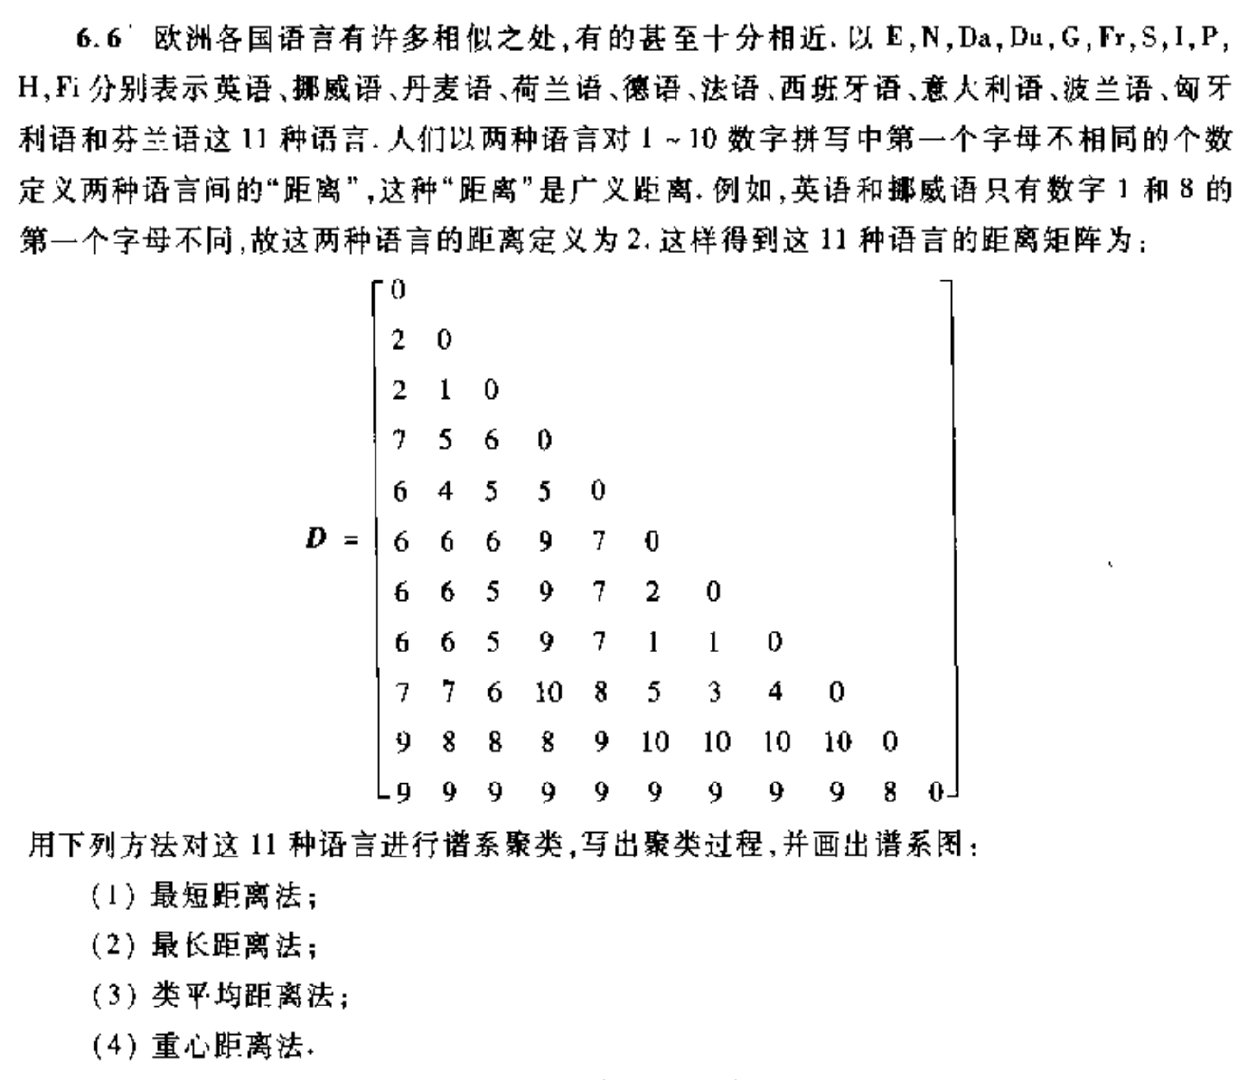
\includegraphics{ex_6_6_files/008i3skNly1grd8hp3zuaj30yx0u0dn0.jpg}
\caption{习题 6.6}
\end{figure}

    \begin{tcolorbox}[breakable, size=fbox, boxrule=1pt, pad at break*=1mm,colback=cellbackground, colframe=cellborder]
\prompt{In}{incolor}{40}{\boxspacing}
\begin{Verbatim}[commandchars=\\\{\}]
\PY{n}{data} \PY{o}{\PYZlt{}\PYZhy{}} \PY{n+nf}{read.csv}\PY{p}{(}\PY{l+s}{\PYZdq{}}\PY{l+s}{ex\PYZus{}6\PYZus{}6.csv\PYZdq{}}\PY{p}{,} \PY{n}{header}\PY{o}{=}\PY{k+kc}{TRUE}\PY{p}{,} \PY{n}{row.names}\PY{o}{=}\PY{l+m}{1}\PY{p}{)}
\end{Verbatim}
\end{tcolorbox}

% \begin{center}
% \begin{tabular}{r|lllllllllll}
%   & E & N & Da & Du & G & Fr & S & I & P & H & Fi\\
% \hline
% 	E & 0 & 0 & 0 &  0 & 0 &  0 &  0 &  0 &  0 & 0 & 0\\
% 	N & 2 & 0 & 0 &  0 & 0 &  0 &  0 &  0 &  0 & 0 & 0\\
% 	Da & 2 & 1 & 0 &  0 & 0 &  0 &  0 &  0 &  0 & 0 & 0\\
% 	Du & 7 & 5 & 6 &  0 & 0 &  0 &  0 &  0 &  0 & 0 & 0\\
% 	G & 6 & 4 & 5 &  5 & 0 &  0 &  0 &  0 &  0 & 0 & 0\\
% 	Fr & 6 & 6 & 6 &  9 & 7 &  0 &  0 &  0 &  0 & 0 & 0\\
% 	S & 6 & 6 & 5 &  9 & 7 &  2 &  0 &  0 &  0 & 0 & 0\\
% 	I & 6 & 6 & 5 &  9 & 7 &  1 &  1 &  0 &  0 & 0 & 0\\
% 	P & 7 & 7 & 6 & 10 & 8 &  5 &  3 &  4 &  0 & 0 & 0\\
% 	H & 9 & 8 & 8 &  8 & 9 & 10 & 10 & 10 & 10 & 0 & 0\\
% 	Fi & 9 & 9 & 9 &  9 & 9 &  9 &  9 &  9 &  9 & 8 & 0\\
% \end{tabular}
% \end{center}

计算距离:
    
    \begin{tcolorbox}[breakable, size=fbox, boxrule=1pt, pad at break*=1mm,colback=cellbackground, colframe=cellborder]
\prompt{In}{incolor}{43}{\boxspacing}
\begin{Verbatim}[commandchars=\\\{\}]
\PY{n}{d} \PY{o}{\PYZlt{}\PYZhy{}} \PY{n+nf}{as.dist}\PY{p}{(}\PY{n}{data}\PY{p}{)}\PY{p}{;} \PY{n}{d}    \PY{c+c1}{\PYZsh{} dist: 距离}
\end{Verbatim}
\end{tcolorbox}

    
    \begin{Verbatim}[commandchars=\\\{\}]
    E  N Da Du  G Fr  S  I  P  H
N   2                           
Da  2  1                        
Du  7  5  6                     
G   6  4  5  5                  
Fr  6  6  6  9  7               
S   6  6  5  9  7  2            
I   6  6  5  9  7  1  1         
P   7  7  6 10  8  5  3  4      
H   9  8  8  8  9 10 10 10 10   
Fi  9  9  9  9  9  9  9  9  9  8
    \end{Verbatim}

    
    \hypertarget{ux6700ux77edux8dddux79bb}{%
\subsection{(1) 最短距离法}\label{ux6700ux77edux8dddux79bb}}

    \begin{tcolorbox}[breakable, size=fbox, boxrule=1pt, pad at break*=1mm,colback=cellbackground, colframe=cellborder]
\prompt{In}{incolor}{52}{\boxspacing}
\begin{Verbatim}[commandchars=\\\{\}]
\PY{n}{h1} \PY{o}{\PYZlt{}\PYZhy{}} \PY{n+nf}{hclust}\PY{p}{(}\PY{n}{d}\PY{p}{,} \PY{l+s}{\PYZdq{}}\PY{l+s}{single\PYZdq{}}\PY{p}{)}
\end{Verbatim}
\end{tcolorbox}

画出谱系图:

    \begin{tcolorbox}[breakable, size=fbox, boxrule=1pt, pad at break*=1mm,colback=cellbackground, colframe=cellborder]
\prompt{In}{incolor}{67}{\boxspacing}
\begin{Verbatim}[commandchars=\\\{\}]
\PY{n+nf}{plot}\PY{p}{(}\PY{n}{h1}\PY{p}{,} \PY{n}{hang}\PY{o}{=}\PY{l+m}{\PYZhy{}1}\PY{p}{,} \PY{n}{main}\PY{o}{=}\PY{l+s}{\PYZdq{}}\PY{l+s}{Shortest Distance Cluster\PYZdq{}}\PY{p}{,} \PY{n}{xlab}\PY{o}{=}\PY{l+s}{\PYZdq{}}\PY{l+s}{Language\PYZdq{}}\PY{p}{)}    \PY{c+c1}{\PYZsh{} hang=\PYZhy{}1 表示线画到底}
\end{Verbatim}
\end{tcolorbox}

    \begin{center}
    \adjustimage{max size={0.6\linewidth}{0.6\paperheight}}{ex_6_6_files/ex_6_6_5_0.png}
    \end{center}
    
聚类过程:

首先在距离为1的时候,将挪威语和丹麦语聚为一类,得新类CL10=\{丹麦语,挪威语\},
其中包含2个样本,这是全部类被分为类;
然后,将法语和意大利语聚为一类,CL9=\{法语,意大利语\};
其中包含两个样本,这是全部样本被分为9类;
接着在最短距离为2的时候,波兰语被分到CL9当中,
也即CL8=\{CL9,波兰语\},
然后英语被分到CL10中,的新类CL7=\{CL10,英语\}=\{丹麦语,挪威语,英语\},$\cdots$ 
如此继续下去,直到距离为8的时候,所有语言合为一类,聚类结束。 

    \hypertarget{ux6700ux957fux8dddux79bb}{%
\subsection{(2) 最长距离法}\label{ux6700ux957fux8dddux79bb}}

    \begin{tcolorbox}[breakable, size=fbox, boxrule=1pt, pad at break*=1mm,colback=cellbackground, colframe=cellborder]
\prompt{In}{incolor}{68}{\boxspacing}
\begin{Verbatim}[commandchars=\\\{\}]
\PY{n}{h2} \PY{o}{\PYZlt{}\PYZhy{}} \PY{n+nf}{hclust}\PY{p}{(}\PY{n}{d}\PY{p}{,} \PY{l+s}{\PYZdq{}}\PY{l+s}{complete\PYZdq{}}\PY{p}{)}
\PY{n+nf}{plot}\PY{p}{(}\PY{n}{h2}\PY{p}{,} \PY{n}{hang}\PY{o}{=}\PY{l+m}{\PYZhy{}1}\PY{p}{,} \PY{n}{main}\PY{o}{=}\PY{l+s}{\PYZdq{}}\PY{l+s}{Longest Distance Cluster\PYZdq{}}\PY{p}{,} \PY{n}{xlab}\PY{o}{=}\PY{l+s}{\PYZdq{}}\PY{l+s}{Language\PYZdq{}}\PY{p}{)}
\end{Verbatim}
\end{tcolorbox}

    \begin{center}
    \adjustimage{max size={0.6\linewidth}{0.5\paperheight}}{ex_6_6_files/ex_6_6_7_0.png}
    \end{center}
    
    \hypertarget{ux7c7bux5e73ux5747ux8dddux79bb}{%
\subsection{(3) 类平均距离法}\label{ux7c7bux5e73ux5747ux8dddux79bb}}

    \begin{tcolorbox}[breakable, size=fbox, boxrule=1pt, pad at break*=1mm,colback=cellbackground, colframe=cellborder]
\prompt{In}{incolor}{69}{\boxspacing}
\begin{Verbatim}[commandchars=\\\{\}]
\PY{n}{h3} \PY{o}{\PYZlt{}\PYZhy{}} \PY{n+nf}{hclust}\PY{p}{(}\PY{n}{d}\PY{p}{,} \PY{l+s}{\PYZdq{}}\PY{l+s}{average\PYZdq{}}\PY{p}{)}
\PY{n+nf}{plot}\PY{p}{(}\PY{n}{h3}\PY{p}{,} \PY{n}{hang}\PY{o}{=}\PY{l+m}{\PYZhy{}1}\PY{p}{,} \PY{n}{main}\PY{o}{=}\PY{l+s}{\PYZdq{}}\PY{l+s}{Classes Average Distance Cluster\PYZdq{}}\PY{p}{,} \PY{n}{xlab}\PY{o}{=}\PY{l+s}{\PYZdq{}}\PY{l+s}{Language\PYZdq{}}\PY{p}{)}
\end{Verbatim}
\end{tcolorbox}

    \begin{center}
    \adjustimage{max size={0.6\linewidth}{0.5\paperheight}}{ex_6_6_files/ex_6_6_9_0.png}
    \end{center}
    
    \hypertarget{ux91cdux5fc3ux8dddux79bb}{%
\subsection{(4) 重心距离法}\label{ux91cdux5fc3ux8dddux79bb}}

    \begin{tcolorbox}[breakable, size=fbox, boxrule=1pt, pad at break*=1mm,colback=cellbackground, colframe=cellborder]
\prompt{In}{incolor}{70}{\boxspacing}
\begin{Verbatim}[commandchars=\\\{\}]
\PY{n}{h4} \PY{o}{\PYZlt{}\PYZhy{}} \PY{n+nf}{hclust}\PY{p}{(}\PY{n}{d}\PY{p}{,} \PY{l+s}{\PYZdq{}}\PY{l+s}{centroid\PYZdq{}}\PY{p}{)}
\PY{n+nf}{plot}\PY{p}{(}\PY{n}{h4}\PY{p}{,} \PY{n}{hang}\PY{o}{=}\PY{l+m}{\PYZhy{}1}\PY{p}{,} \PY{n}{main}\PY{o}{=}\PY{l+s}{\PYZdq{}}\PY{l+s}{Centroid Distance Cluster\PYZdq{}}\PY{p}{,} \PY{n}{xlab}\PY{o}{=}\PY{l+s}{\PYZdq{}}\PY{l+s}{Language\PYZdq{}}\PY{p}{)}
\end{Verbatim}
\end{tcolorbox}

    \begin{center}
    \adjustimage{max size={0.6\linewidth}{0.6\paperheight}}{ex_6_6_files/ex_6_6_11_0.png}
    \end{center}
    


%%%%%%%%%%%%%%%%%%%%%%%%%%%%%%%%
% - MARK: 6.7
%%%%%%%%%%%%%%%%%%%%%%%%%%%%%%%%


    
    \hypertarget{ux4e60ux9898-6.7}{%
\section{习题 6.7}\label{ux4e60ux9898-6.7}}


\includegraphics{ex_6_7_files/008i3skNly1gre3npqkfbj31a209e0we.jpg}

\includegraphics{ex_6_7_files/008i3skNly1gre3o642hfj31j40a2gov.jpg}

    \begin{tcolorbox}[breakable, size=fbox, boxrule=1pt, pad at break*=1mm,colback=cellbackground, colframe=cellborder]
\prompt{In}{incolor}{1}{\boxspacing}
\begin{Verbatim}[commandchars=\\\{\}]
\PY{n}{data} \PY{o}{\PYZlt{}\PYZhy{}} \PY{n+nf}{read.csv}\PY{p}{(}\PY{l+s}{\PYZdq{}}\PY{l+s}{ex\PYZus{}6\PYZus{}7.csv\PYZdq{}}\PY{p}{,} \PY{n}{row.names}\PY{o}{=}\PY{l+m}{1}\PY{p}{)}\PY{p}{;} \PY{n}{data}
\end{Verbatim}
\end{tcolorbox}

    A data.frame: 16 × 6
\begin{tabular}{r|llllll}
  & x1 & x2 & x3 & x4 & x5 & x6\\
  & <dbl> & <dbl> & <dbl> & <dbl> & <dbl> & <dbl>\\
\hline
	1985 & 128.1 & 100.0 & 134.2 & 100.0 & 166.8 & 111.1\\
	1986 & 135.8 & 106.5 & 143.6 & 106.1 & 177.5 & 114.7\\
    \vdots\\
	1999 & 359.8 & 329.7 & 472.8 & 314.3 & 424.3 & 280.5\\
	2000 & 354.4 & 331.0 & 476.6 & 314.0 & 409.0 & 277.1\\
\end{tabular}

计算得到距离:
    
    \begin{tcolorbox}[breakable, size=fbox, boxrule=1pt, pad at break*=1mm,colback=cellbackground, colframe=cellborder]
\prompt{In}{incolor}{2}{\boxspacing}
\begin{Verbatim}[commandchars=\\\{\}]
\PY{n}{d} \PY{o}{\PYZlt{}\PYZhy{}} \PY{n+nf}{dist}\PY{p}{(}\PY{n}{data}\PY{p}{)}
\end{Verbatim}
\end{tcolorbox}

将距离代入 hclust 函数即可完成聚类。

    \hypertarget{ux6700ux957fux8dddux79bbux6cd5}{%
\subsection{(1) 最长距离法}\label{ux6700ux957fux8dddux79bbux6cd5}}

    \begin{tcolorbox}[breakable, size=fbox, boxrule=1pt, pad at break*=1mm,colback=cellbackground, colframe=cellborder]
\prompt{In}{incolor}{3}{\boxspacing}
\begin{Verbatim}[commandchars=\\\{\}]
\PY{n}{h1} \PY{o}{\PYZlt{}\PYZhy{}} \PY{n+nf}{hclust}\PY{p}{(}\PY{n}{d}\PY{p}{,} \PY{n}{method}\PY{o}{=}\PY{l+s}{\PYZdq{}}\PY{l+s}{complete\PYZdq{}}\PY{p}{)}

\PY{n+nf}{plot}\PY{p}{(}\PY{n}{h1}\PY{p}{,} \PY{n}{hang}\PY{o}{=}\PY{l+m}{\PYZhy{}1}\PY{p}{,} \PY{n}{main}\PY{o}{=}\PY{l+s}{\PYZdq{}}\PY{l+s}{Longest Distance Cluster\PYZdq{}}\PY{p}{,} \PY{n}{xlab}\PY{o}{=}\PY{l+s}{\PYZdq{}}\PY{l+s}{Year\PYZdq{}}\PY{p}{)}    \PY{c+c1}{\PYZsh{} hang=\PYZhy{}1 表示线画到底}
\PY{n+nf}{rect.hclust}\PY{p}{(}\PY{n}{h1}\PY{p}{,} \PY{n}{k}\PY{o}{=}\PY{l+m}{3}\PY{p}{)}    \PY{c+c1}{\PYZsh{} 画出分为 3 类的矩形框}
\end{Verbatim}
\end{tcolorbox}

    \begin{center}
    \adjustimage{max size={0.9\linewidth}{0.9\paperheight}}{ex_6_7_files/ex_6_7_4_0.png}
    \end{center}
    
    可以看出聚成三类的结果是:

\begin{itemize}
\tightlist
\item
  第一类:1994,1999,2000,1995,1998,1996,1997
\item
  第二类:1988,1987,1985,1986
\item
  第三类:1993,1989,1990,1991,1992
\end{itemize}

    \hypertarget{ux7c7bux5e73ux5747ux8dddux79bbux6cd5}{%
\subsection{(2)
类平均距离法}\label{ux7c7bux5e73ux5747ux8dddux79bbux6cd5}}

    \begin{tcolorbox}[breakable, size=fbox, boxrule=1pt, pad at break*=1mm,colback=cellbackground, colframe=cellborder]
\prompt{In}{incolor}{5}{\boxspacing}
\begin{Verbatim}[commandchars=\\\{\}]
\PY{n}{h2} \PY{o}{\PYZlt{}\PYZhy{}} \PY{n+nf}{hclust}\PY{p}{(}\PY{n}{d}\PY{p}{,} \PY{n}{method}\PY{o}{=}\PY{l+s}{\PYZdq{}}\PY{l+s}{average\PYZdq{}}\PY{p}{)}
\PY{n+nf}{plot}\PY{p}{(}\PY{n}{h2}\PY{p}{,} \PY{n}{hang}\PY{o}{=}\PY{l+m}{\PYZhy{}1}\PY{p}{,} \PY{n}{main}\PY{o}{=}\PY{l+s}{\PYZdq{}}\PY{l+s}{Classes Average Distance Cluster\PYZdq{}}\PY{p}{,} \PY{n}{xlab}\PY{o}{=}\PY{l+s}{\PYZdq{}}\PY{l+s}{Year\PYZdq{}}\PY{p}{)}
\PY{n+nf}{rect.hclust}\PY{p}{(}\PY{n}{h2}\PY{p}{,} \PY{n}{k}\PY{o}{=}\PY{l+m}{3}\PY{p}{)}    \PY{c+c1}{\PYZsh{} 画出分为 3 类的矩形框}
\end{Verbatim}
\end{tcolorbox}

    \begin{center}
    \adjustimage{max size={0.9\linewidth}{0.9\paperheight}}{ex_6_7_files/ex_6_7_8_0.png}
    \end{center}
    
    聚成三类的结果是:

\begin{itemize}
\tightlist
\item
  第一类:1994,1999,2000,1995,1998,1996,1997
\item
  第二类:1987,1985,1986
\item
  第三类:1993,1988,1992,1991,1989,1990
\end{itemize}

    \hypertarget{ux6570ux636eux6807ux51c6ux5316}{%
\subsection{(3) 数据标准化}\label{ux6570ux636eux6807ux51c6ux53165}}

    \hypertarget{ux6570ux636eux6807ux51c6ux5316}{%
\subsubsection{数据标准化}\label{ux6570ux636eux6807ux51c6ux53164}}

    先用 scale 将数据标准化:

    \begin{tcolorbox}[breakable, size=fbox, boxrule=1pt, pad at break*=1mm,colback=cellbackground, colframe=cellborder]
\prompt{In}{incolor}{7}{\boxspacing}
\begin{Verbatim}[commandchars=\\\{\}]
\PY{n}{data.scale} \PY{o}{\PYZlt{}\PYZhy{}} \PY{n+nf}{scale}\PY{p}{(}\PY{n}{data}\PY{p}{)}\PY{p}{;} \PY{n}{data.scale}
\end{Verbatim}
\end{tcolorbox}

% \begin{tabular}{r|llllll}
%   & x1 & x2 & x3 & x4 & x5 & x6\\
% \hline
% 	1985 & -1.41939946 & -1.3334326 & -1.3213620 & -1.3417390 & -1.3788101 & -1.40310086\\
% 	1986 & -1.33797367 & -1.2628375 & -1.2521774 & -1.2707383 & -1.2972638 & -1.35108734\\
% 	1987 & -1.23328338 & -1.1781234 & -1.1594406 & -1.1939179 & -1.1349331 & -1.27162223\\
% 	1988 & -0.94776440 & -0.9446166 & -0.9217104 & -0.9646205 & -0.7866463 & -1.00722017\\
% 	1989 & -0.62311874 & -0.6796135 & -0.6957563 & -0.6678142 & -0.5069498 & -0.63301178\\
% 	1990 & -0.57764720 & -0.6253096 & -0.6751482 & -0.5840100 & -0.5625843 & -0.52320546\\
% 	1991 & -0.51419854 & -0.5644892 & -0.5919794 & -0.5397801 & -0.6045006 & -0.44807481\\
% 	1992 & -0.39258860 & -0.4461067 & -0.4440420 & -0.4478283 & -0.5351481 & -0.36860971\\
% 	1993 & -0.07851772 & -0.1561238 & -0.1437513 & -0.1661533 & -0.2516411 & -0.05652858\\
% 	1994 &  0.50626745 &  0.3890875 &  0.3979496 &  0.3809014 &  0.7055762 &  0.45060325\\
% 	1995 &  0.99164972 &  0.8691341 &  0.8528018 &  0.8860541 &  1.3731895 &  0.95917990\\
% 	1996 &  1.22112239 &  1.1417398 &  1.1310123 &  1.1537617 &  1.5423792 &  1.20479931\\
% 	1997 &  1.25284672 &  1.2416590 &  1.2377333 &  1.2457135 &  1.3533745 &  1.25103355\\
% 	1998 &  1.14815642 &  1.2123349 &  1.2163891 &  1.2084672 &  1.0332859 &  1.15712025\\
% 	1999 &  1.03077640 &  1.1612892 &  1.1707567 &  1.1525978 &  0.5836377 &  1.04442428\\
% 	2000 &  0.97367260 &  1.1754082 &  1.1987249 &  1.1491059 &  0.4670340 &  0.99530040\\
% \end{tabular}


    
    重新计算标准化数据的距离:

    \begin{tcolorbox}[breakable, size=fbox, boxrule=1pt, pad at break*=1mm,colback=cellbackground, colframe=cellborder]
\prompt{In}{incolor}{8}{\boxspacing}
\begin{Verbatim}[commandchars=\\\{\}]
\PY{n}{ds} \PY{o}{\PYZlt{}\PYZhy{}} \PY{n+nf}{dist}\PY{p}{(}\PY{n}{data.scale}\PY{p}{)}
\end{Verbatim}
\end{tcolorbox}

    \hypertarget{ux6700ux957fux8dddux79bbux6cd5}{%
\subsubsection{最长距离法}\label{ux6700ux957fux8dddux79bbux6cd52}}

    \begin{tcolorbox}[breakable, size=fbox, boxrule=1pt, pad at break*=1mm,colback=cellbackground, colframe=cellborder]
\prompt{In}{incolor}{9}{\boxspacing}
\begin{Verbatim}[commandchars=\\\{\}]
\PY{n}{h3} \PY{o}{\PYZlt{}\PYZhy{}} \PY{n+nf}{hclust}\PY{p}{(}\PY{n}{ds}\PY{p}{,} \PY{n}{method}\PY{o}{=}\PY{l+s}{\PYZdq{}}\PY{l+s}{complete\PYZdq{}}\PY{p}{)}
\PY{n+nf}{plot}\PY{p}{(}\PY{n}{h3}\PY{p}{,} \PY{n}{hang}\PY{o}{=}\PY{l+m}{\PYZhy{}1}\PY{p}{,} \PY{n}{main}\PY{o}{=}\PY{l+s}{\PYZdq{}}\PY{l+s}{Longest Distance Cluster \PYZhy{} scaled data\PYZdq{}}\PY{p}{,} \PY{n}{xlab}\PY{o}{=}\PY{l+s}{\PYZdq{}}\PY{l+s}{Year\PYZdq{}}\PY{p}{)}
\PY{n+nf}{rect.hclust}\PY{p}{(}\PY{n}{h3}\PY{p}{,} \PY{n}{k}\PY{o}{=}\PY{l+m}{3}\PY{p}{)}
\end{Verbatim}
\end{tcolorbox}

    \begin{center}
    \adjustimage{max size={0.9\linewidth}{0.9\paperheight}}{ex_6_7_files/ex_6_7_18_0.png}
    \end{center}

    聚成三类的结果:

\begin{itemize}
\tightlist
\item
  第一类:1994,1999,2000,1995,1998,1996,1997
\item
  第二类:1988,1987,1985,1986
\item
  第三类:1993,1992,1989,1990,1991
\end{itemize}

    \hypertarget{ux7c7bux5e73ux5747ux8dddux79bbux6cd5}{%
\subsubsection{类平均距离法}\label{ux7c7bux5e73ux5747ux8dddux79bbux6cd53}}

    \begin{tcolorbox}[breakable, size=fbox, boxrule=1pt, pad at break*=1mm,colback=cellbackground, colframe=cellborder]
\prompt{In}{incolor}{11}{\boxspacing}
\begin{Verbatim}[commandchars=\\\{\}]
\PY{n}{h4} \PY{o}{\PYZlt{}\PYZhy{}} \PY{n+nf}{hclust}\PY{p}{(}\PY{n}{ds}\PY{p}{,} \PY{n}{method}\PY{o}{=}\PY{l+s}{\PYZdq{}}\PY{l+s}{average\PYZdq{}}\PY{p}{)}

\PY{n+nf}{plot}\PY{p}{(}\PY{n}{h4}\PY{p}{,} \PY{n}{hang}\PY{o}{=}\PY{l+m}{\PYZhy{}1}\PY{p}{,} \PY{n}{main}\PY{o}{=}\PY{l+s}{\PYZdq{}}\PY{l+s}{Classes Average Distance Cluster \PYZhy{} scaled data\PYZdq{}}\PY{p}{,} \PY{n}{xlab}\PY{o}{=}\PY{l+s}{\PYZdq{}}\PY{l+s}{Year\PYZdq{}}\PY{p}{)}
\PY{n+nf}{rect.hclust}\PY{p}{(}\PY{n}{h4}\PY{p}{,} \PY{n}{k}\PY{o}{=}\PY{l+m}{3}\PY{p}{)}
\end{Verbatim}
\end{tcolorbox}

    \begin{center}
    \adjustimage{max size={0.9\linewidth}{0.9\paperheight}}{ex_6_7_files/ex_6_7_22_0.png}
    \end{center}
    
    聚成三类的结果:

\begin{itemize}
\tightlist
\item
  第一类:1994,1999,2000,1995,1998,1996,1997
\item
  第二类:1988,1987,1985,1986
\item
  第三类:1993,1992,1989,1990,1991
\end{itemize}

    可以看到,在数据标准化之前不同聚类方法得到的结果不仅尽相同,而且在标准化前后聚类结果也是不要一样的,但是在数据标准化之后,两种不同的聚类方法得到了相同的结果。
    \cite{ref9}


%%%%%%%%%%%%%%%%%%%%%%%%%%%%%%%%
% - MARK: ref
%%%%%%%%%%%%%%%%%%%%%%%%%%%%%%%%    

\begin{thebibliography}{1}

\bibitem{ref1}梅长林 范金城. 数据分析方法[M]. 高等教育出版社, 2006.
\bibitem{ref2}R-project. An Introduction to R [M/OL]. https://cran.r-project.org/doc/manuals/r-release/R-intro.html
\bibitem{ref3}Tiaaaaa. R语言典型相关分析[OL]. https://blog.csdn.net/Tiaaaaa/article/details/58137522
\bibitem{ref4}佚名. CCA 典型相关分析,计算向量之间的相关系数[OL]. https://rstudio-pubs-static.s3.amazonaws.com/553282\_c1046a4c0b1a40ac9319f51b6207a9d7.html
\bibitem{ref5}DoubleHelix. R语言数据分析与挖掘(第八章):判别分析(3)——费歇尔(Fisher)判别分析[OL]. https://cloud.tencent.com/developer/article/1553504
\bibitem{ref6}Jason. Learn R | 多元统计之判别分析(下)[OL]. https://zhuanlan.zhihu.com/p/23965433
\bibitem{ref7}Roger D. Peng. Exploratory Data Analysis with R: Chapter 10 Plotting and Color in R [M/OL]. https://bookdown.org/rdpeng/exdata/plotting-and-color-in-r.html
\bibitem{ref8}将子无怨. R语言进阶之聚类分析[OL]. https://zhuanlan.zhihu.com/p/140534259
\bibitem{ref9}毕业零距离. 聚类分析原理及R语言实现过程 [OL]. https://www.jianshu.com/p/50cb85285af0

\end{thebibliography}

\end{document}
